\chapter{Performance of the Particle Flow algorithm in data/MC comparison}

To study the performance of the Particle Flow algorithm in Run 2 data/Monte Carlo comparison a  $Z \rightarrow \mu \mu$ decay has been chosen. The used dataset was wildcard and wildcard was used for the Monte Carlo. The chapter explains the choice of decay and gives a overview over the event selection before showing a summary of performance plots. 

\section{The $Z \rightarrow \mu \mu$ decay}
\begin{figure}[h]\centering
\begin{fmffile}{ztomumu}
\begin{fmfgraph*}(50,30) \fmfpen{thin}
  \fmfleft{i1} \fmfright{o1,o2}
  \fmf{wiggly, label=$Z$}{i1,v1}
  \fmf{fermion, label=$\mu$}{v1,o2}
  \fmf{fermion, label=$\overline{\mu}$}{v1,o1}
  \end{fmfgraph*}
\end{fmffile}
\caption{Decay of a Z-Boson to two muons}
\label{decay}
\end{figure}


For this thesis $Z\rightarrow \mu \mu$ events were used. The deay channel of a $Z$ boson into a muon and a antimuon has a crossection of \num{3.366 +- 0.007} \cite{pdg}. The event was chosen for this analysis because the Z boson is very easy to trigger on and it allows a very clear event selection. Furthermore the event has exactly one recoiling jet that analysis can be performed on. 

\section{Event selection}
The criteria for the event selection were no good electrons and exactly two good muons, with opposite charge where good means that the particle passed all selection filters itself. The muons are required to have a transversal momentum greater than \SI{25}{\GeV}. Furthermore the muons are restricted to a central $\eta$ region being $|\eta|<2.4$.

Furthermore a jet is required to have a transversal momentum greater than \SI{20}{\GeV} and is required to be recoiling to the reconstructed Z giving the selection criteria $|\phi_{jet}-\phi_Z|<(\pi - \num0.4)$.
The region of pseudorapidity is limited to  $|\eta|<2.5$ to ake into account the the inner tracking detector covers only this region.

Figure one shows the number of events selected. 

\section{Kinematic variables of muons and jets}

After selecting proper $Z \rightarrow \mu \mu$ events the agreement between data and MC has been studied for the selected objects. This section summarizes the kinematic variables of the muons and the chosen recoiling jet.

\begin{figure}[h]
\centering
\begin{subfigure}[b]{0.5\figwidth}
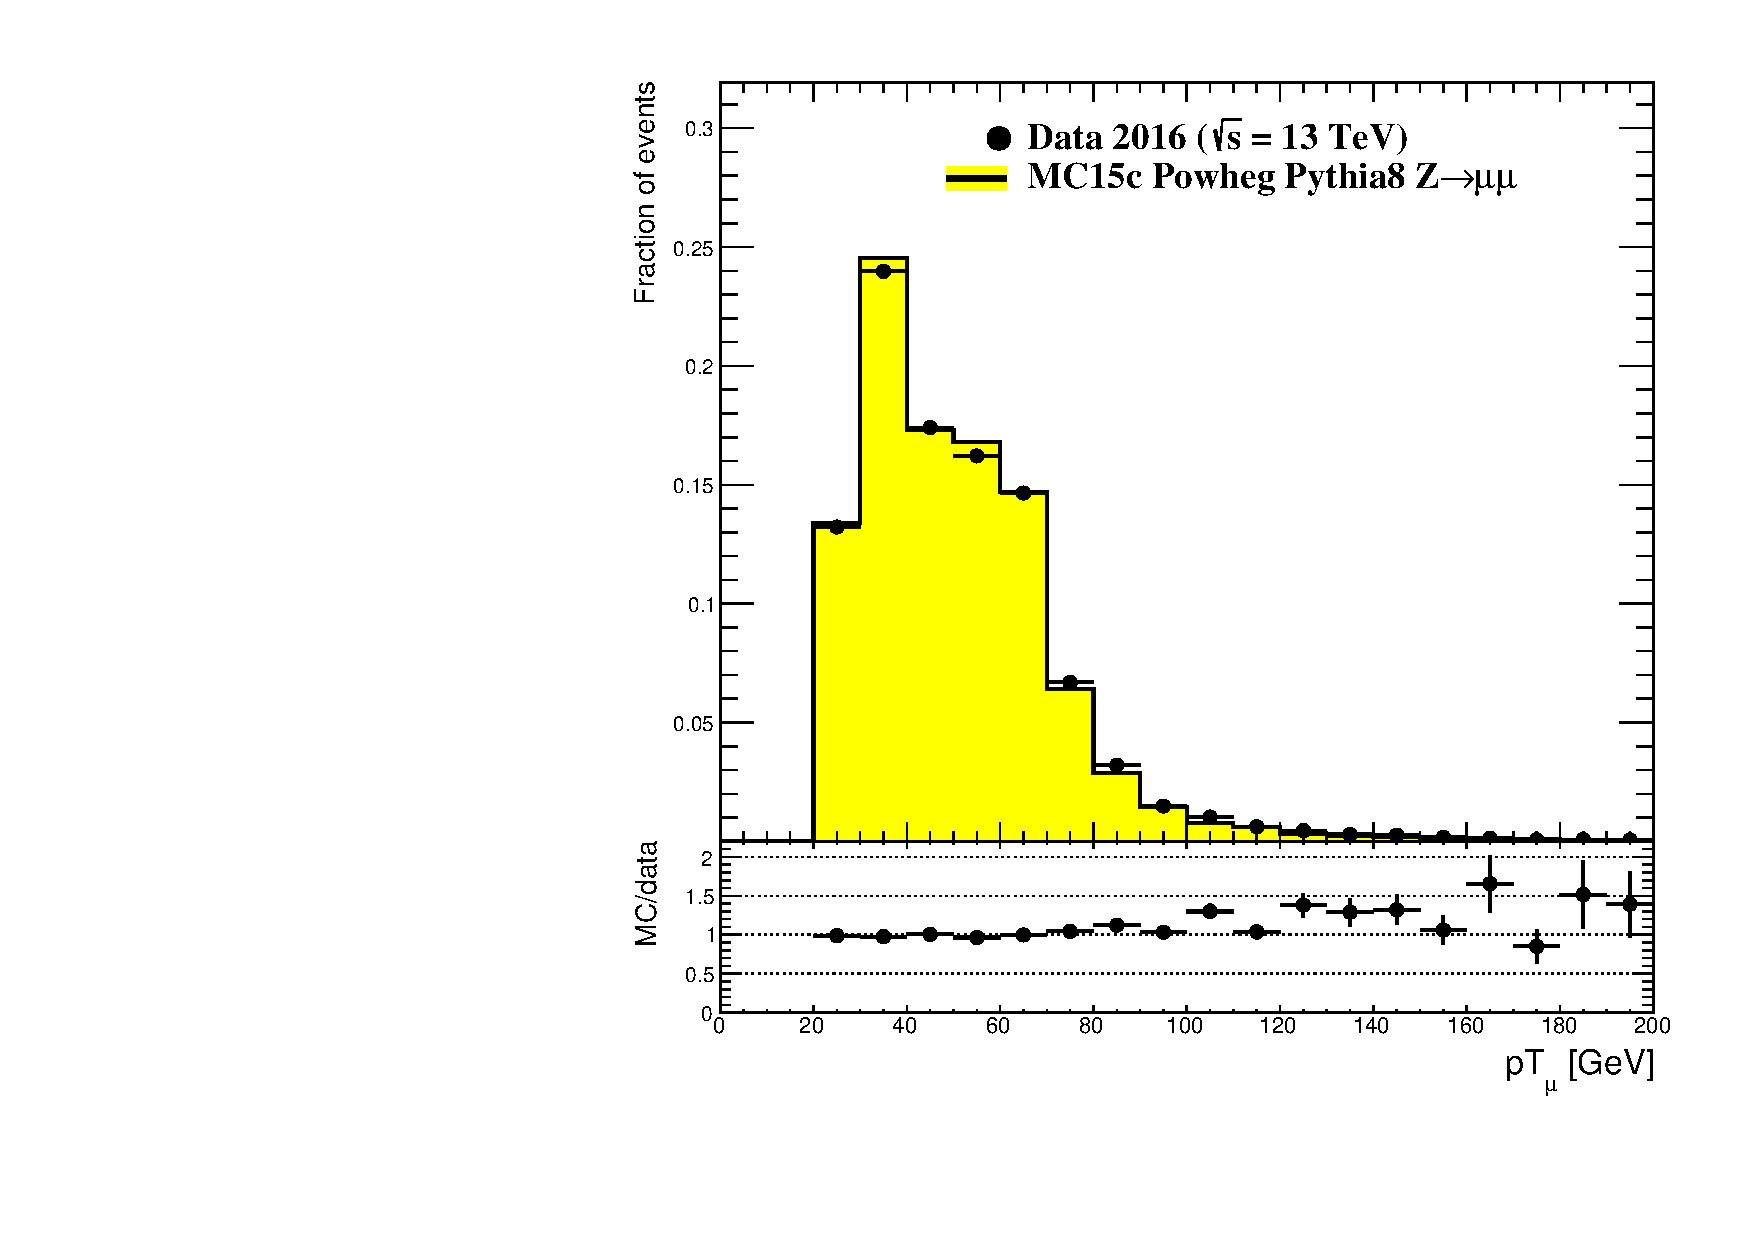
\includegraphics[width=0.53\figwidth]{muon_ptratio}
\caption[Influence of the JES on the transversal momentum]{The influence of the calibration in momentum is shown}
\label{fig:muonpt}
\end{subfigure}
\quad
\begin{subfigure}[b]{0.5\figwidth}
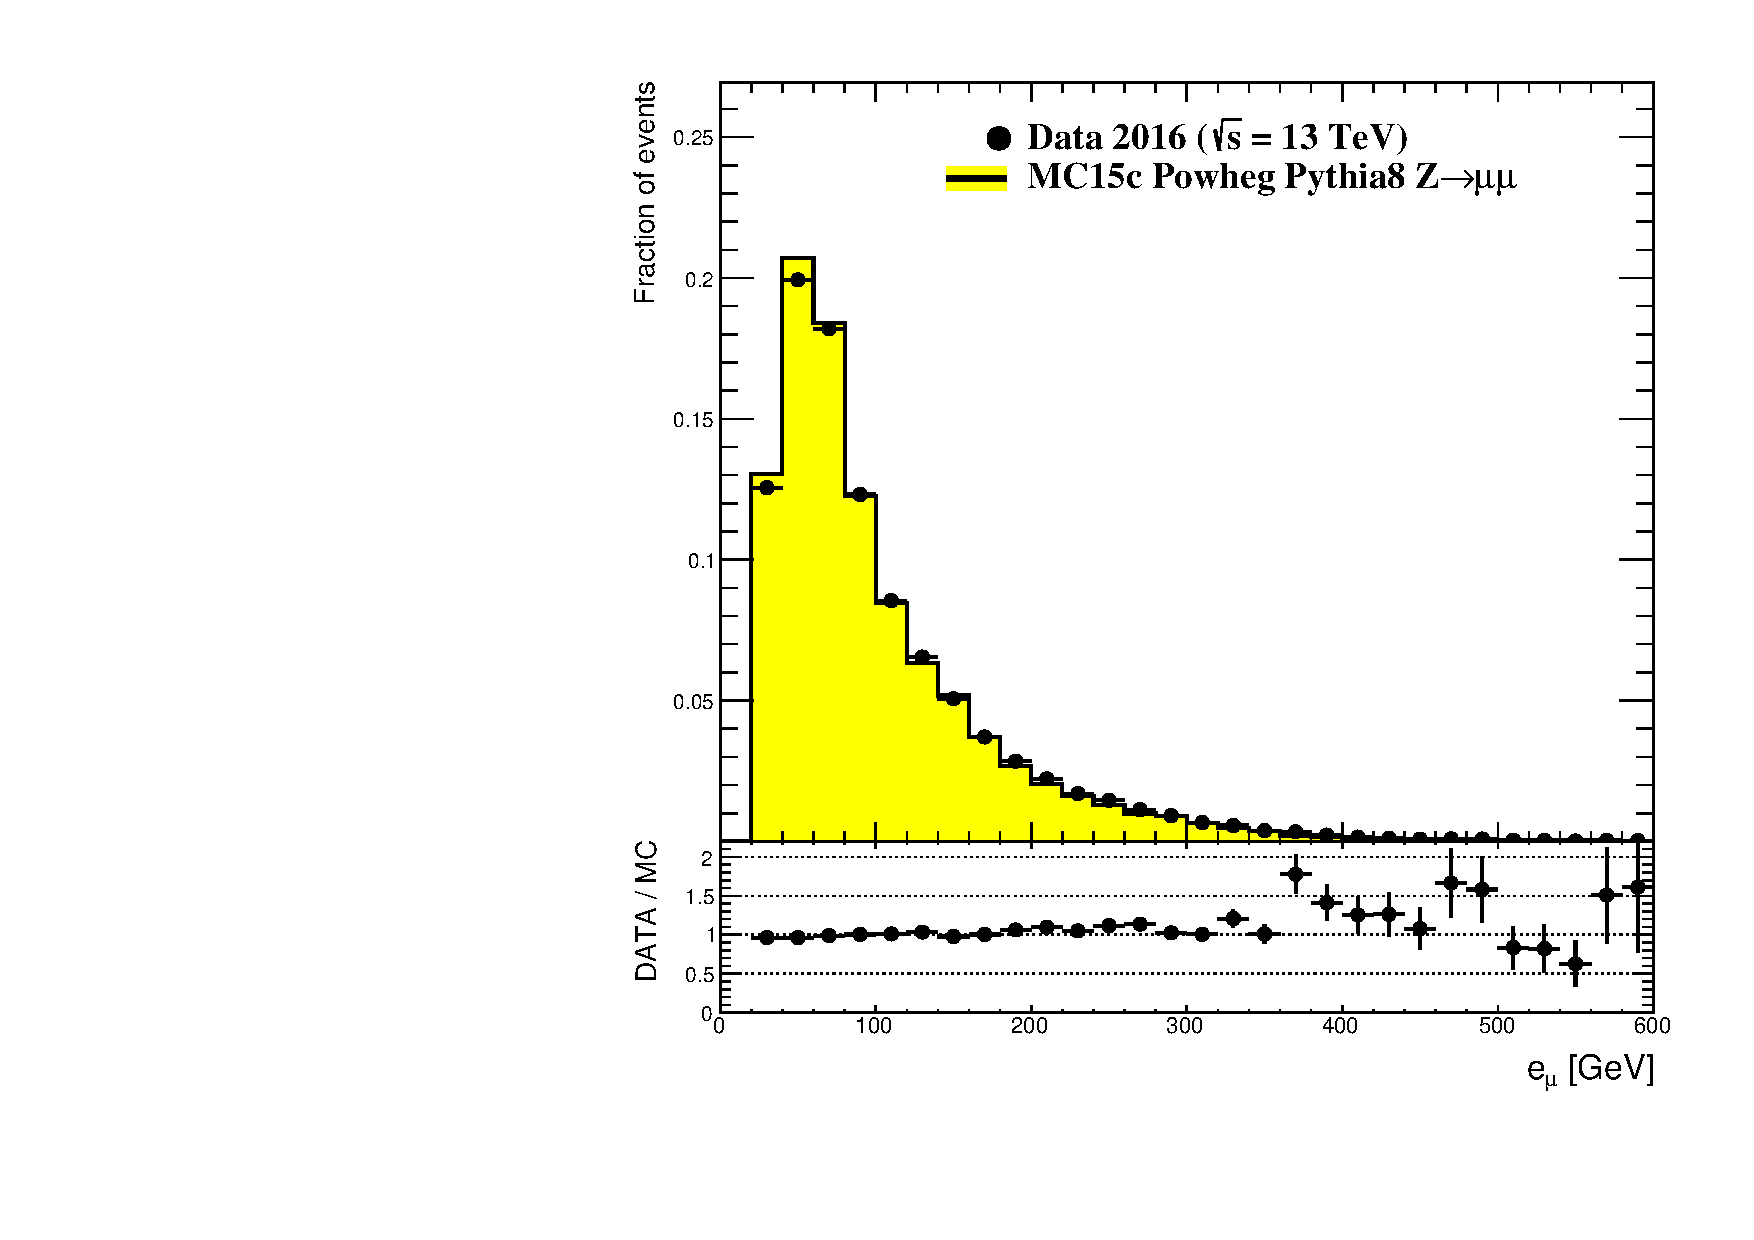
\includegraphics[width=0.53\figwidth]{muon_eratio}
\caption[Influence of the JES on the energy]{The influence of the calibration in energy is shown}
\label{fig:muone}
\end{subfigure}
\end{figure}


\begin{figure}[h]
\centering
\begin{subfigure}[b]{0.5\figwidth}
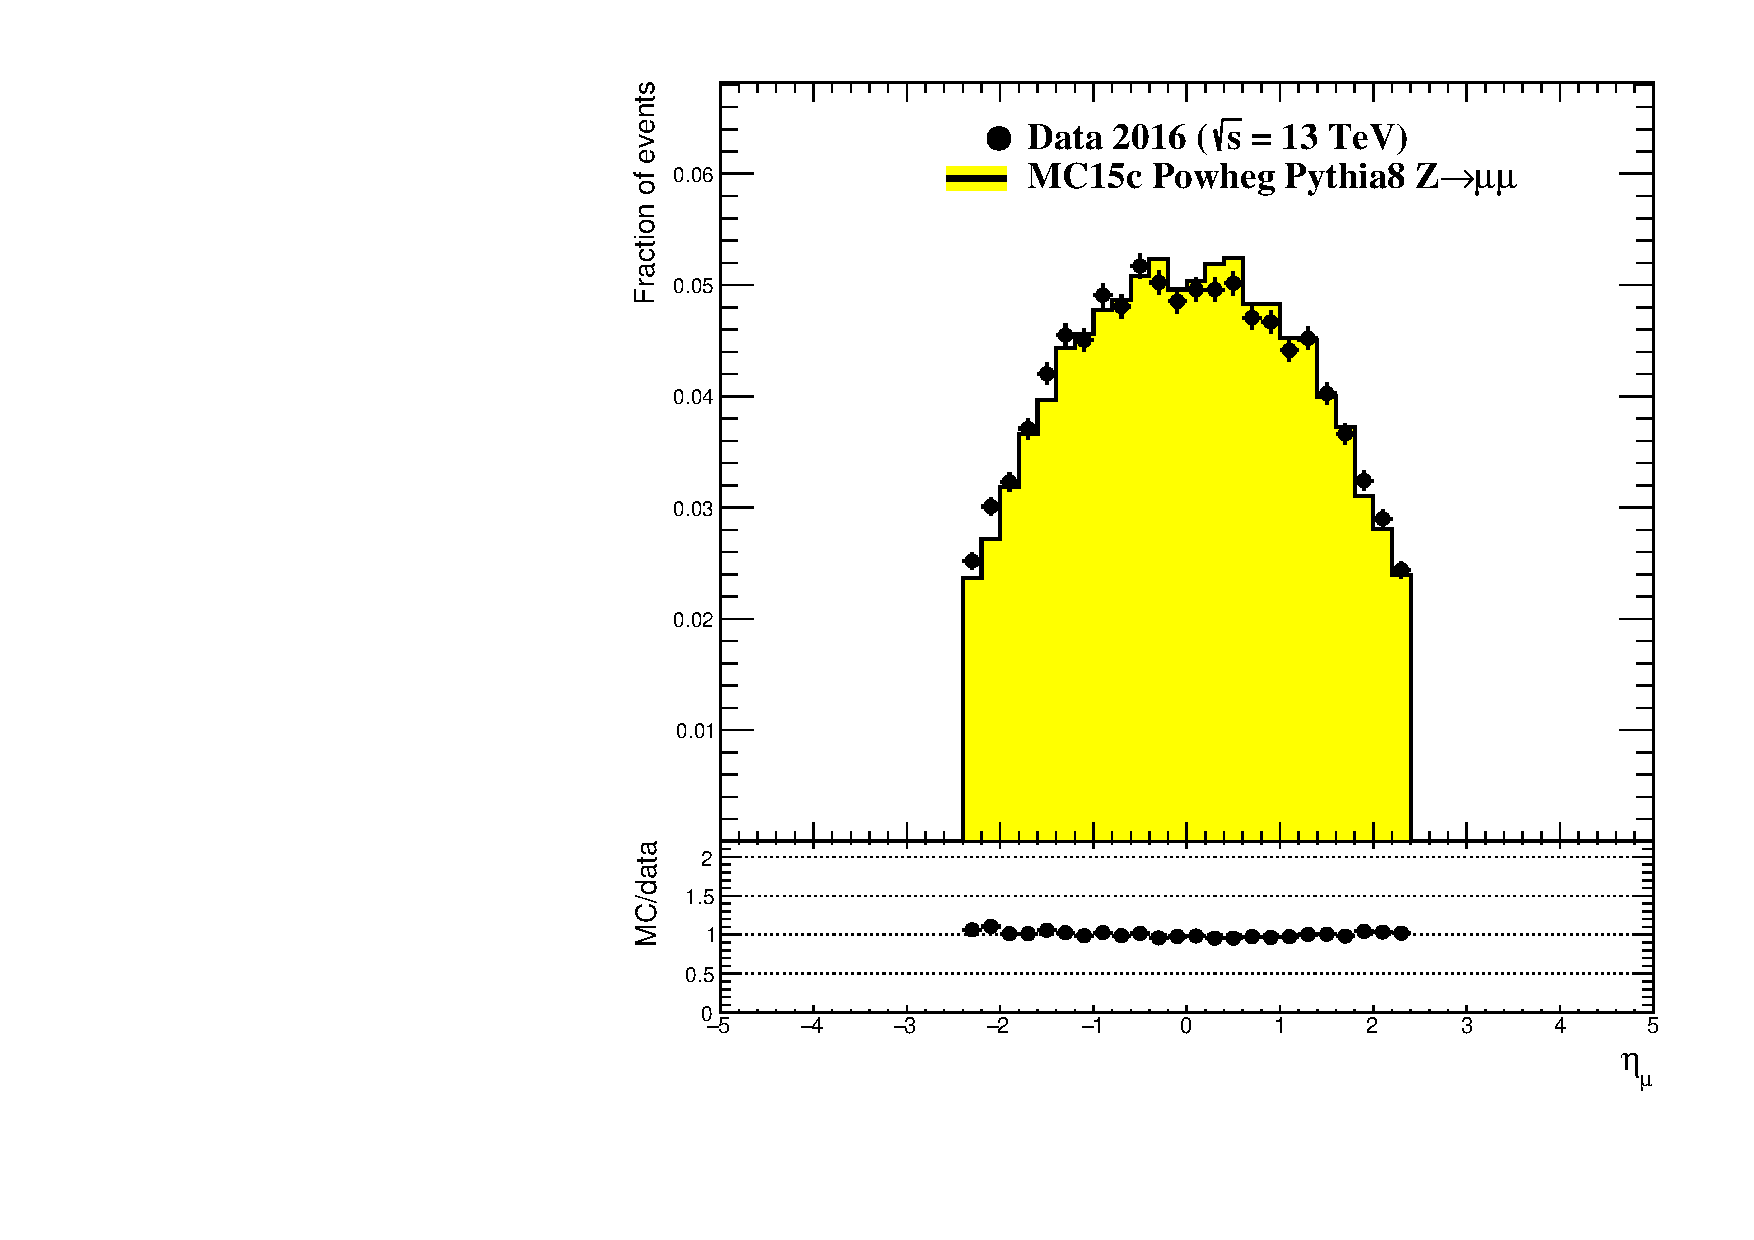
\includegraphics[width=0.53\figwidth]{muon_etaratio}
\caption[Influence of the Smearing on the transversal momentum]{The influence of the Smearing in momentum is shown}
\label{fig:muoneta}
\end{subfigure}
\quad
\begin{subfigure}[b]{0.5\figwidth}
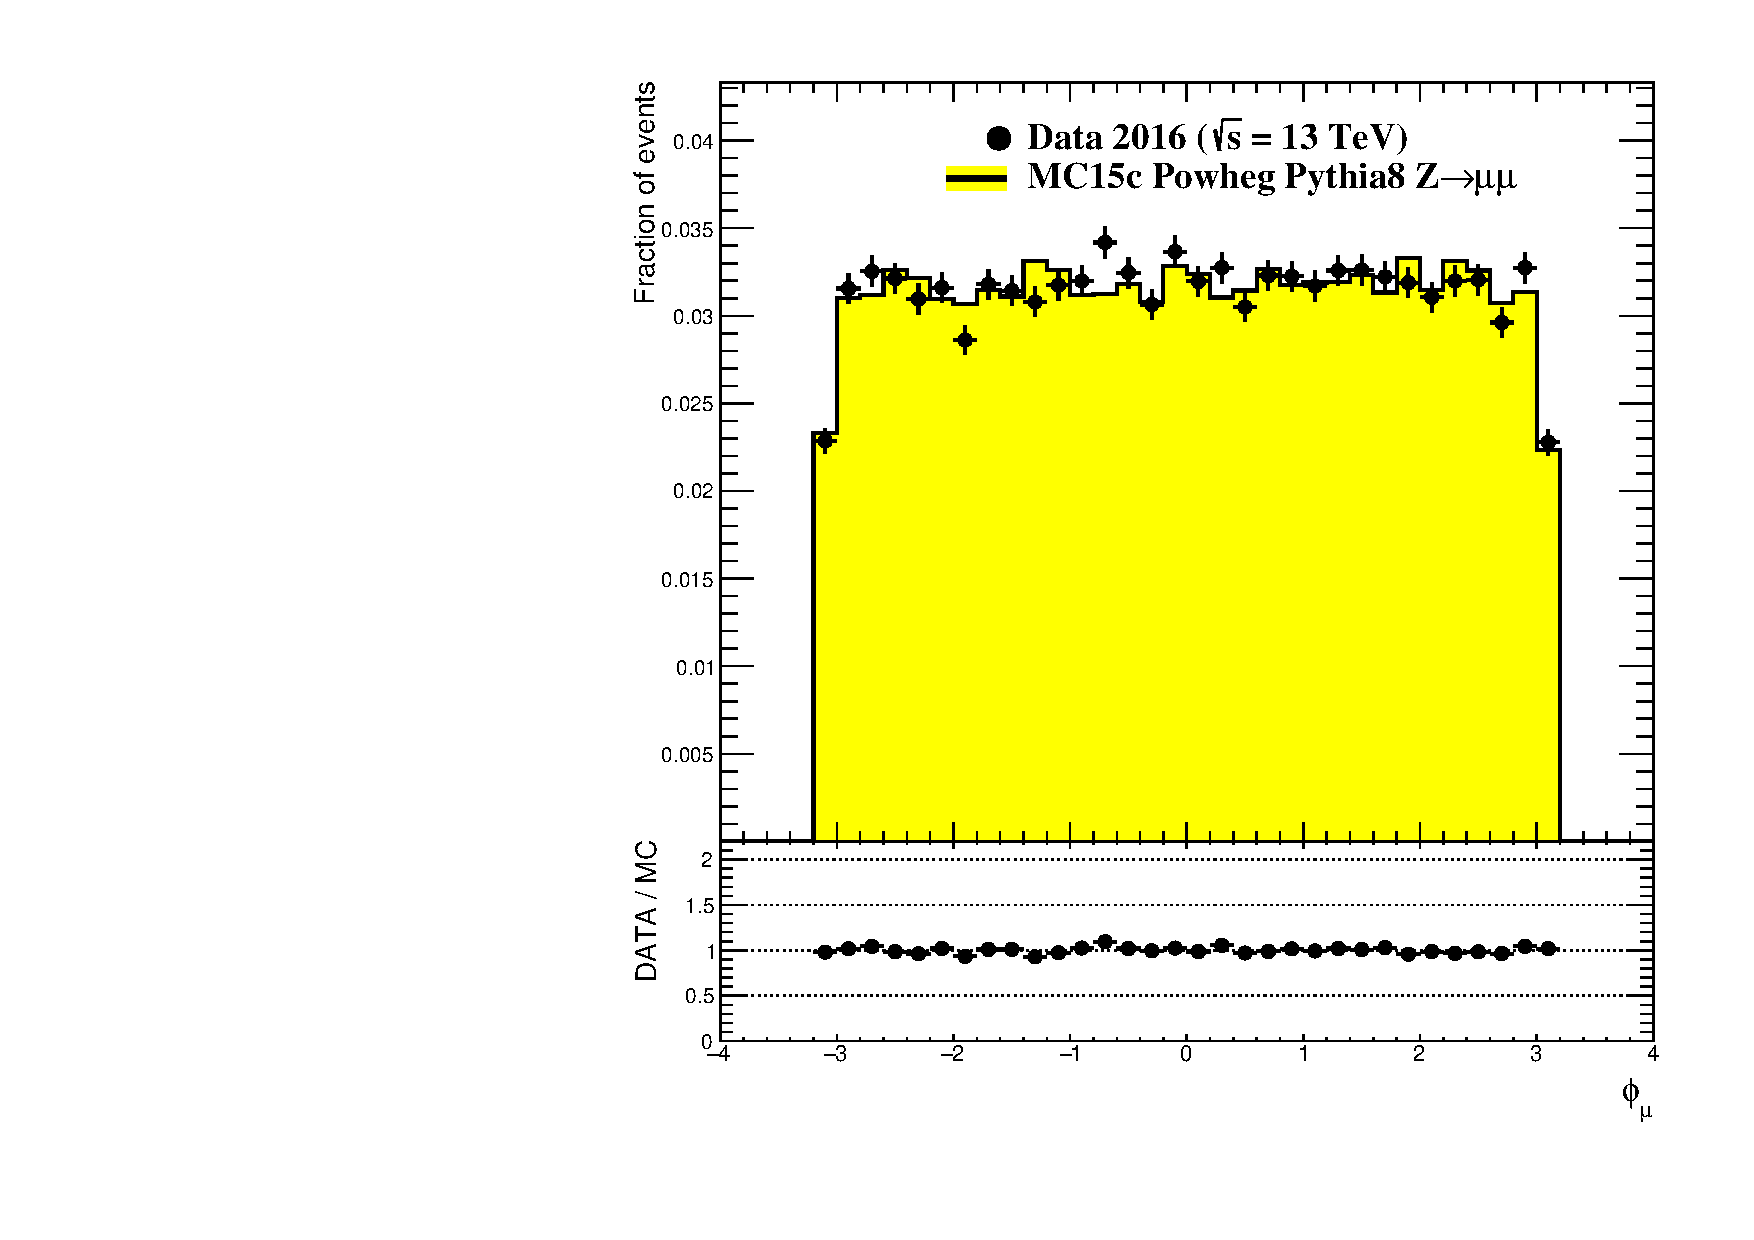
\includegraphics[width=0.53\figwidth]{muon_phiratio}
\caption[Influence of the Smearing on the energy]{The influence of the Smearing in energy is shown}
\label{fig:muonphi}
\end{subfigure}
\end{figure}


\begin{figure}[h]
\centering
\begin{subfigure}[b]{0.5\figwidth}
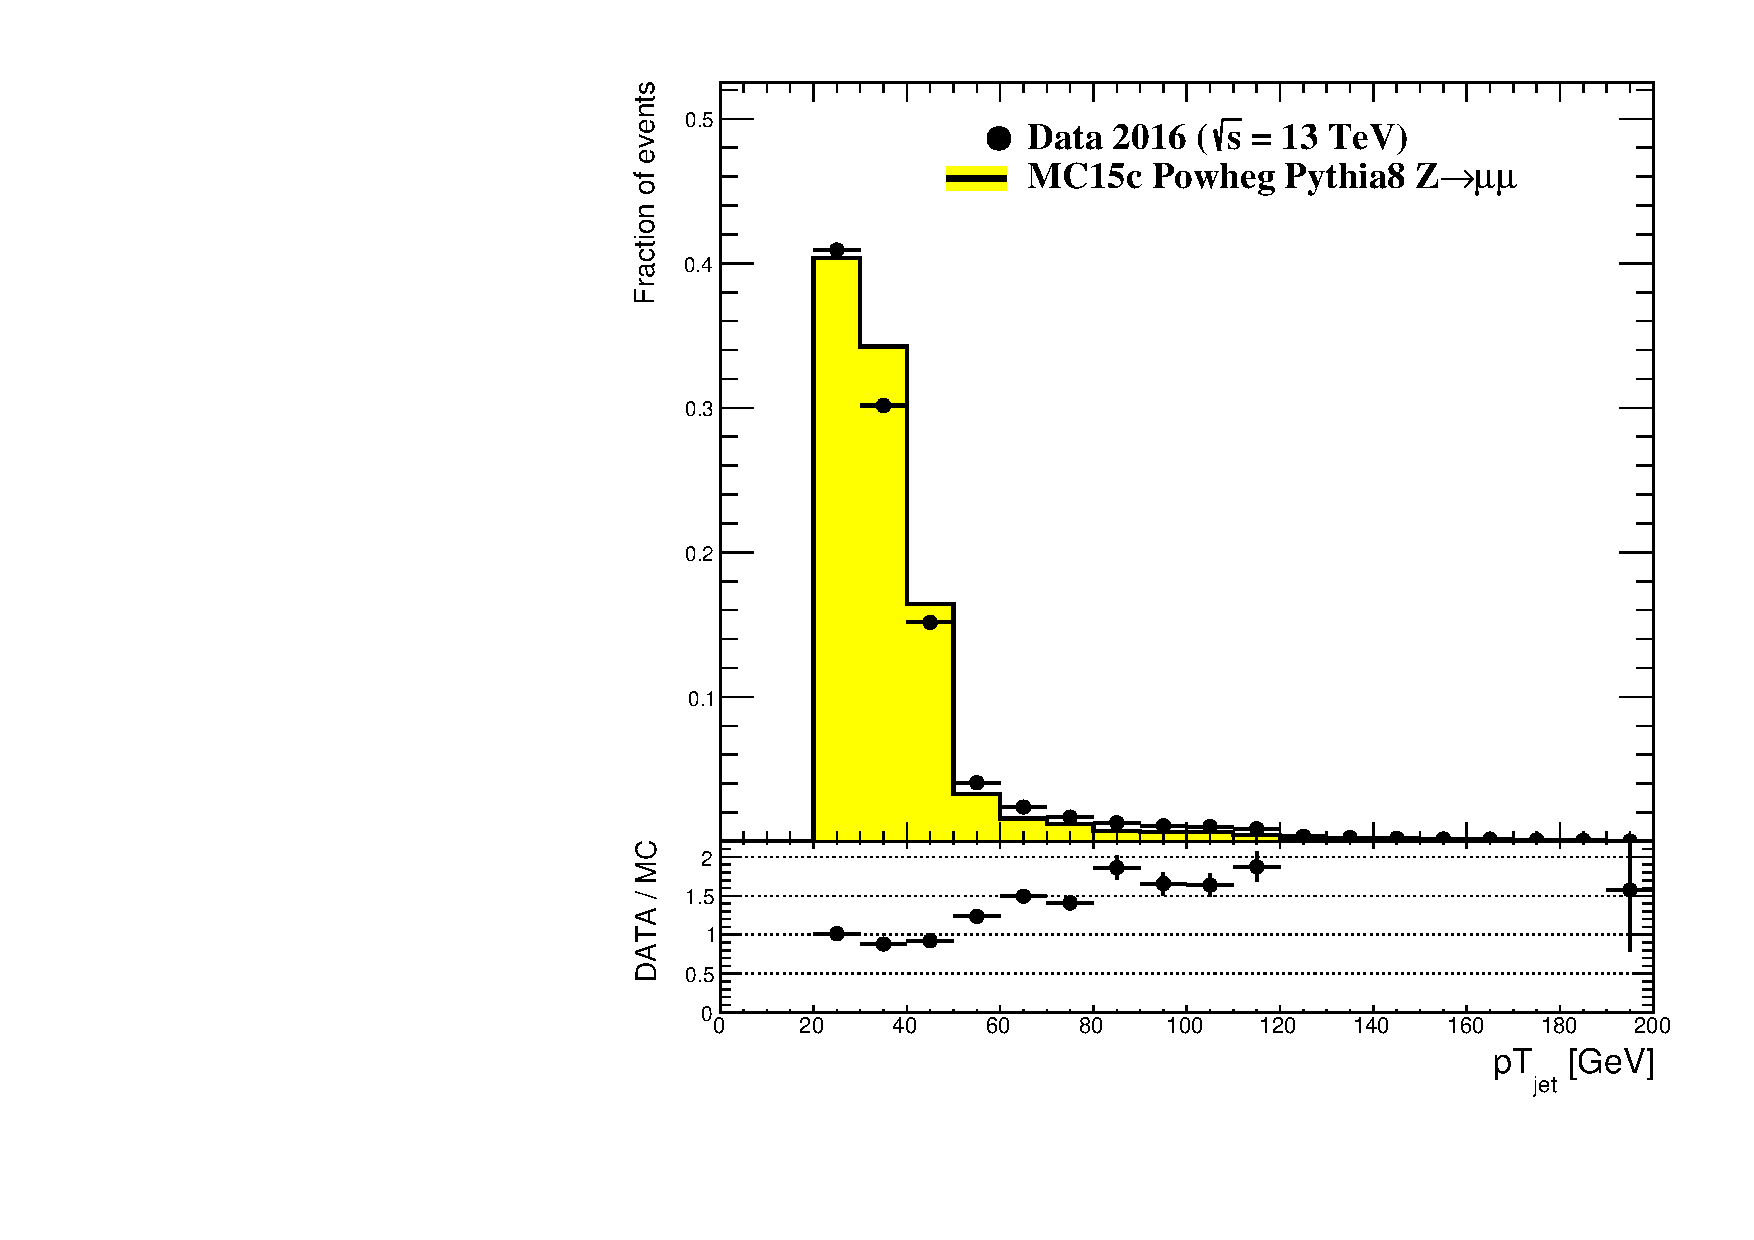
\includegraphics[width=0.53\figwidth]{jet_ptratio}
\caption[Influence of the JES on the transversal momentum]{The influence of the calibration in momentum is shown}
\label{fig:jetpt}
\end{subfigure}
\quad
\begin{subfigure}[b]{0.5\figwidth}
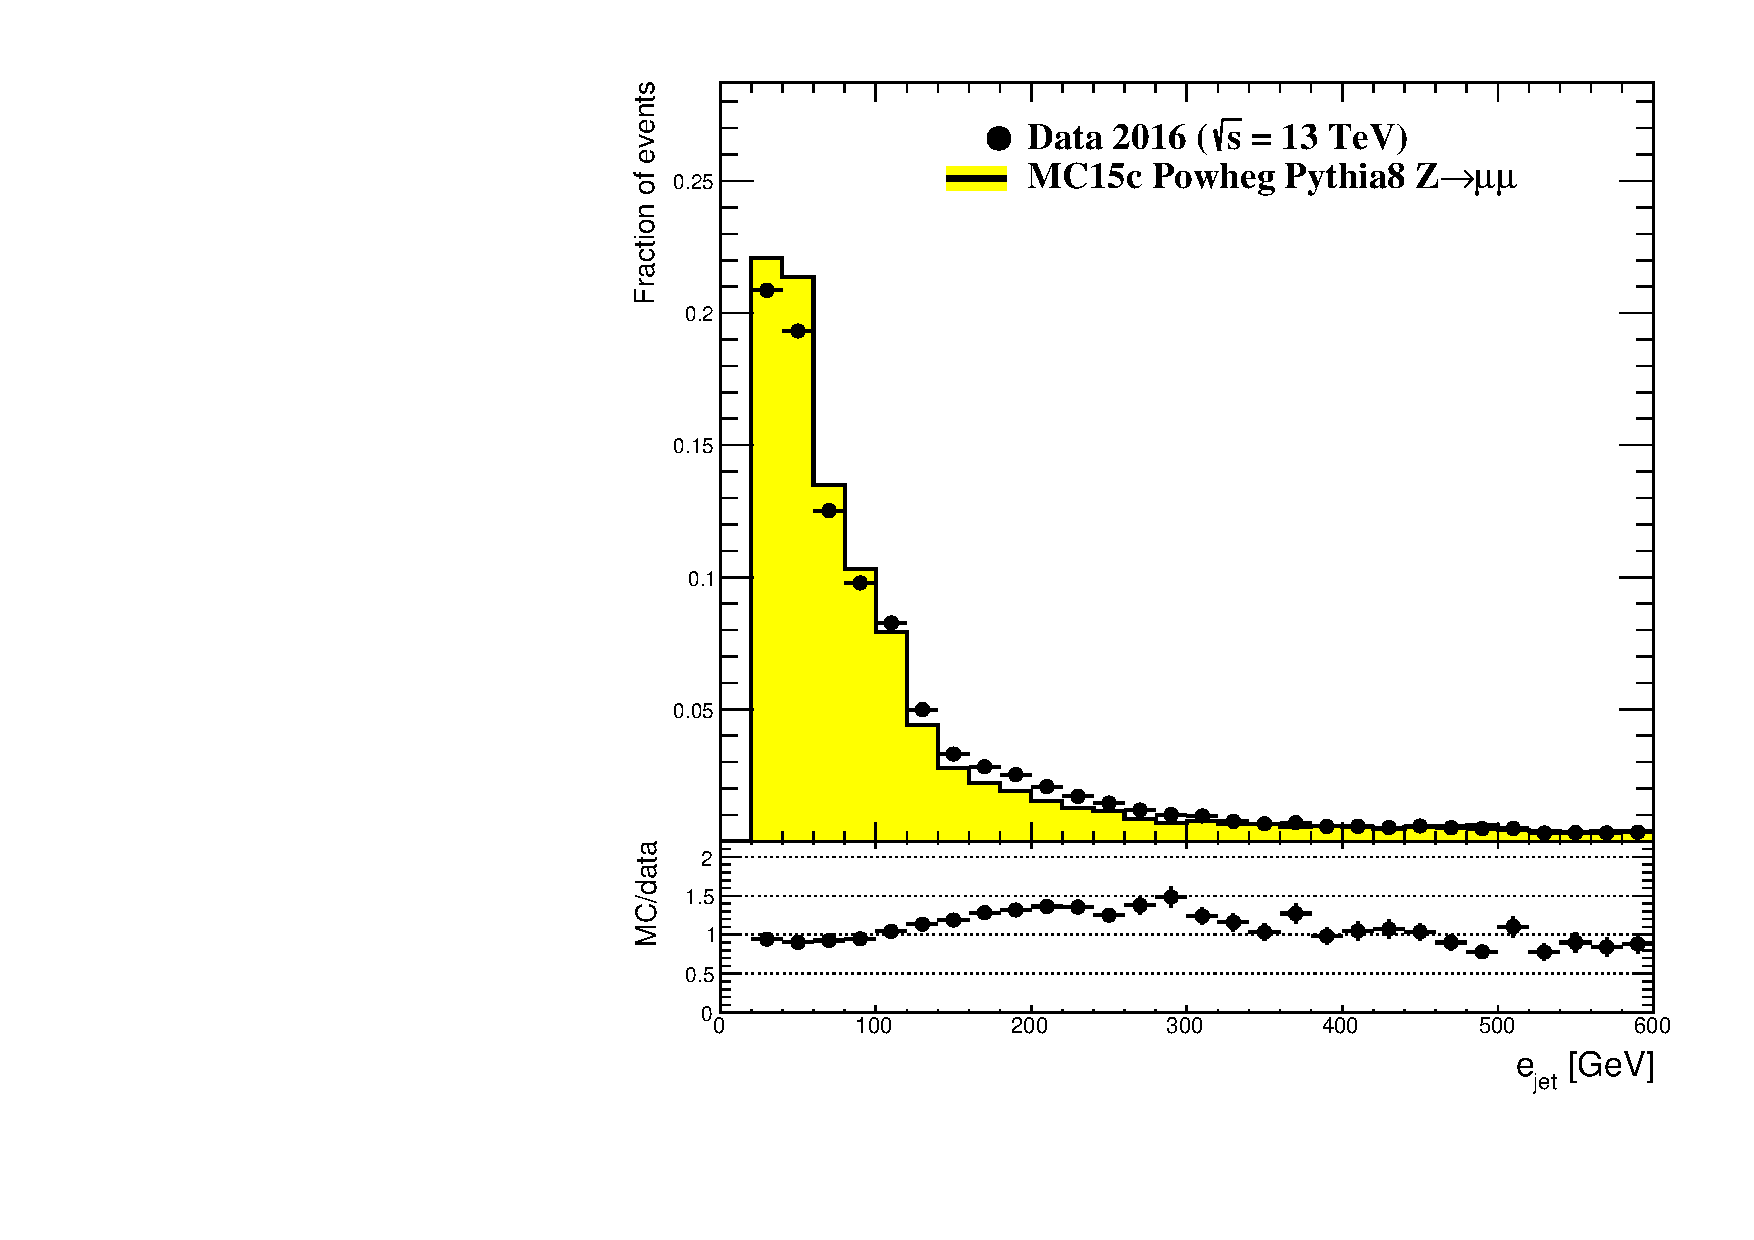
\includegraphics[width=0.53\figwidth]{jet_eratio}
\caption[Influence of the JES on the energy]{The influence of the calibration in energy is shown}
\label{fig:jete}
\end{subfigure}
\end{figure}


\begin{figure}[h]
\centering
\begin{subfigure}[b]{0.5\figwidth}
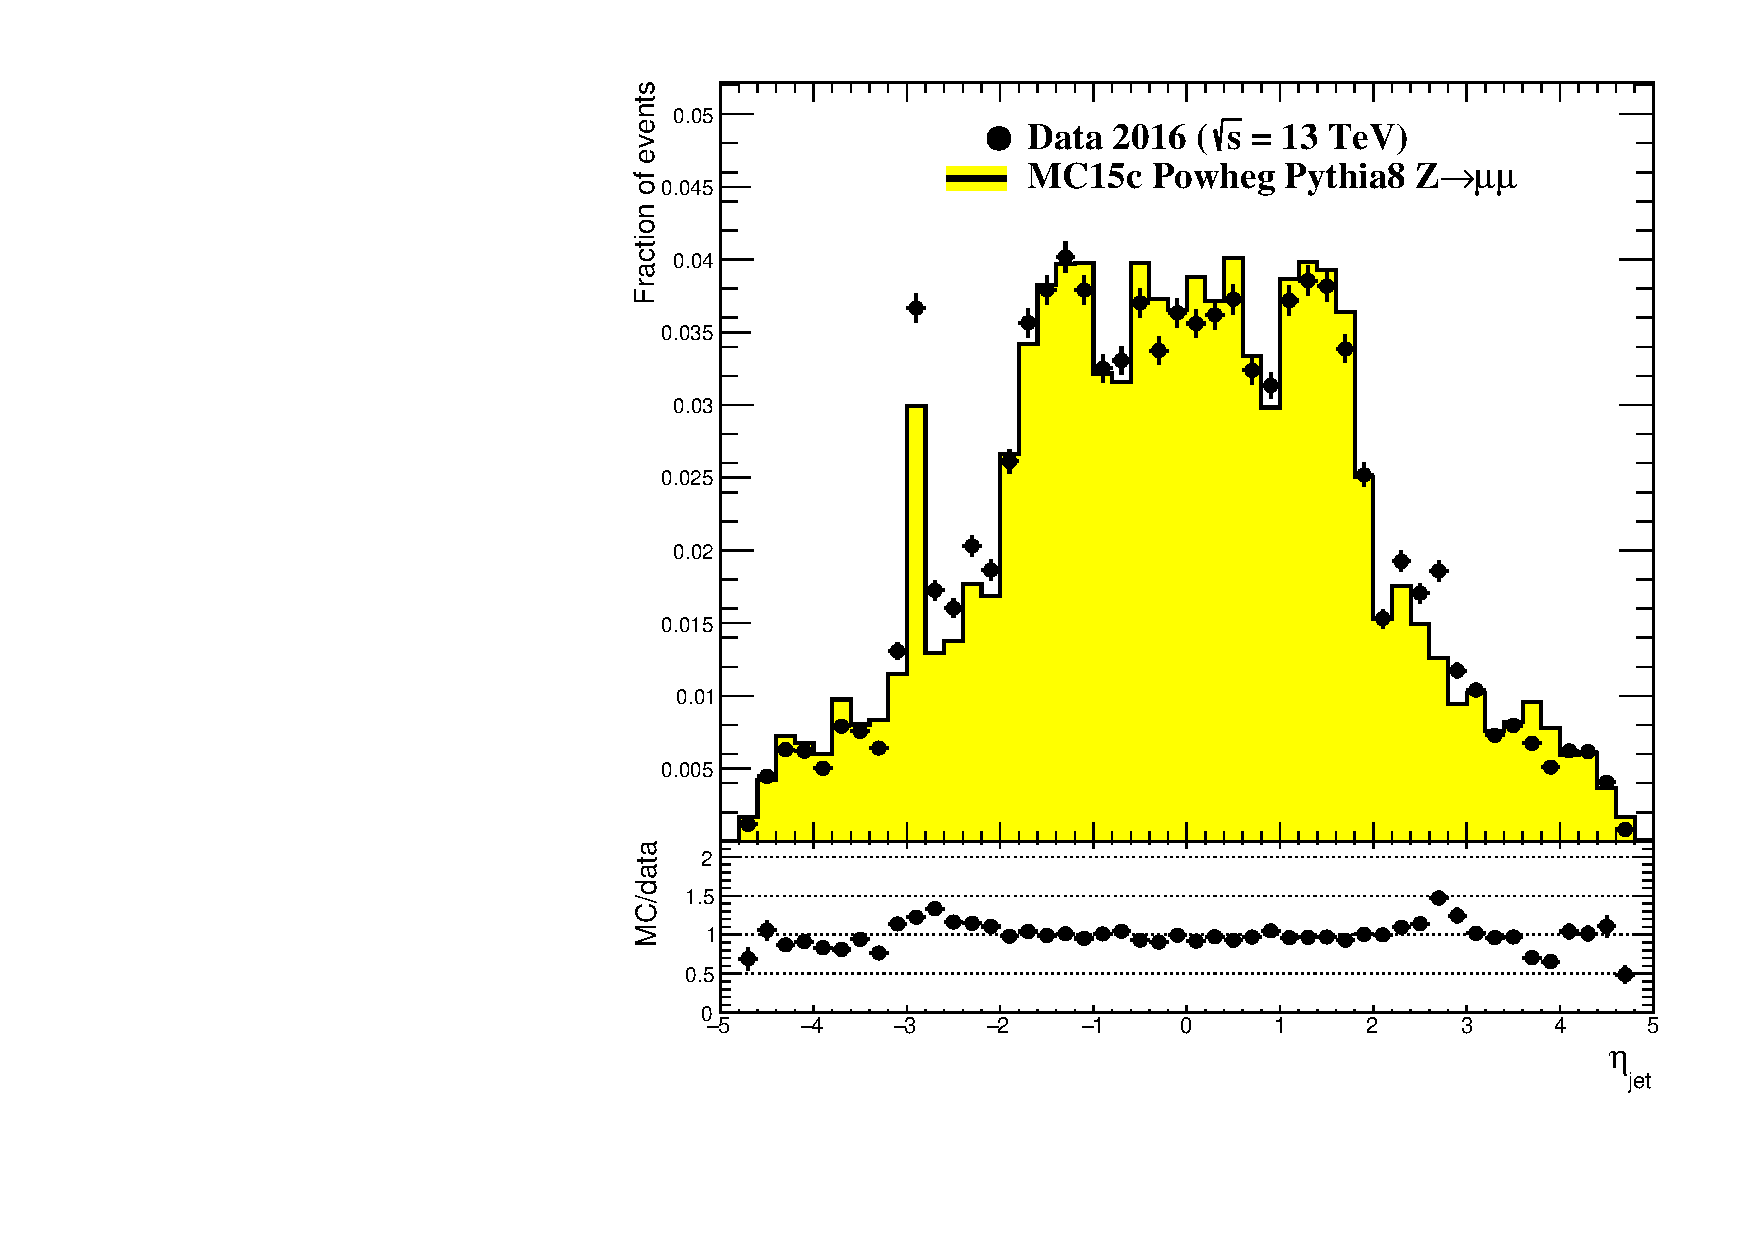
\includegraphics[width=0.53\figwidth]{jet_etaratio}
\caption[Influence of the Smearing on the transversal momentum]{The influence of the Smearing in momentum is shown}
\label{fig:jeteta}
\end{subfigure}
\quad
\begin{subfigure}[b]{0.5\figwidth}
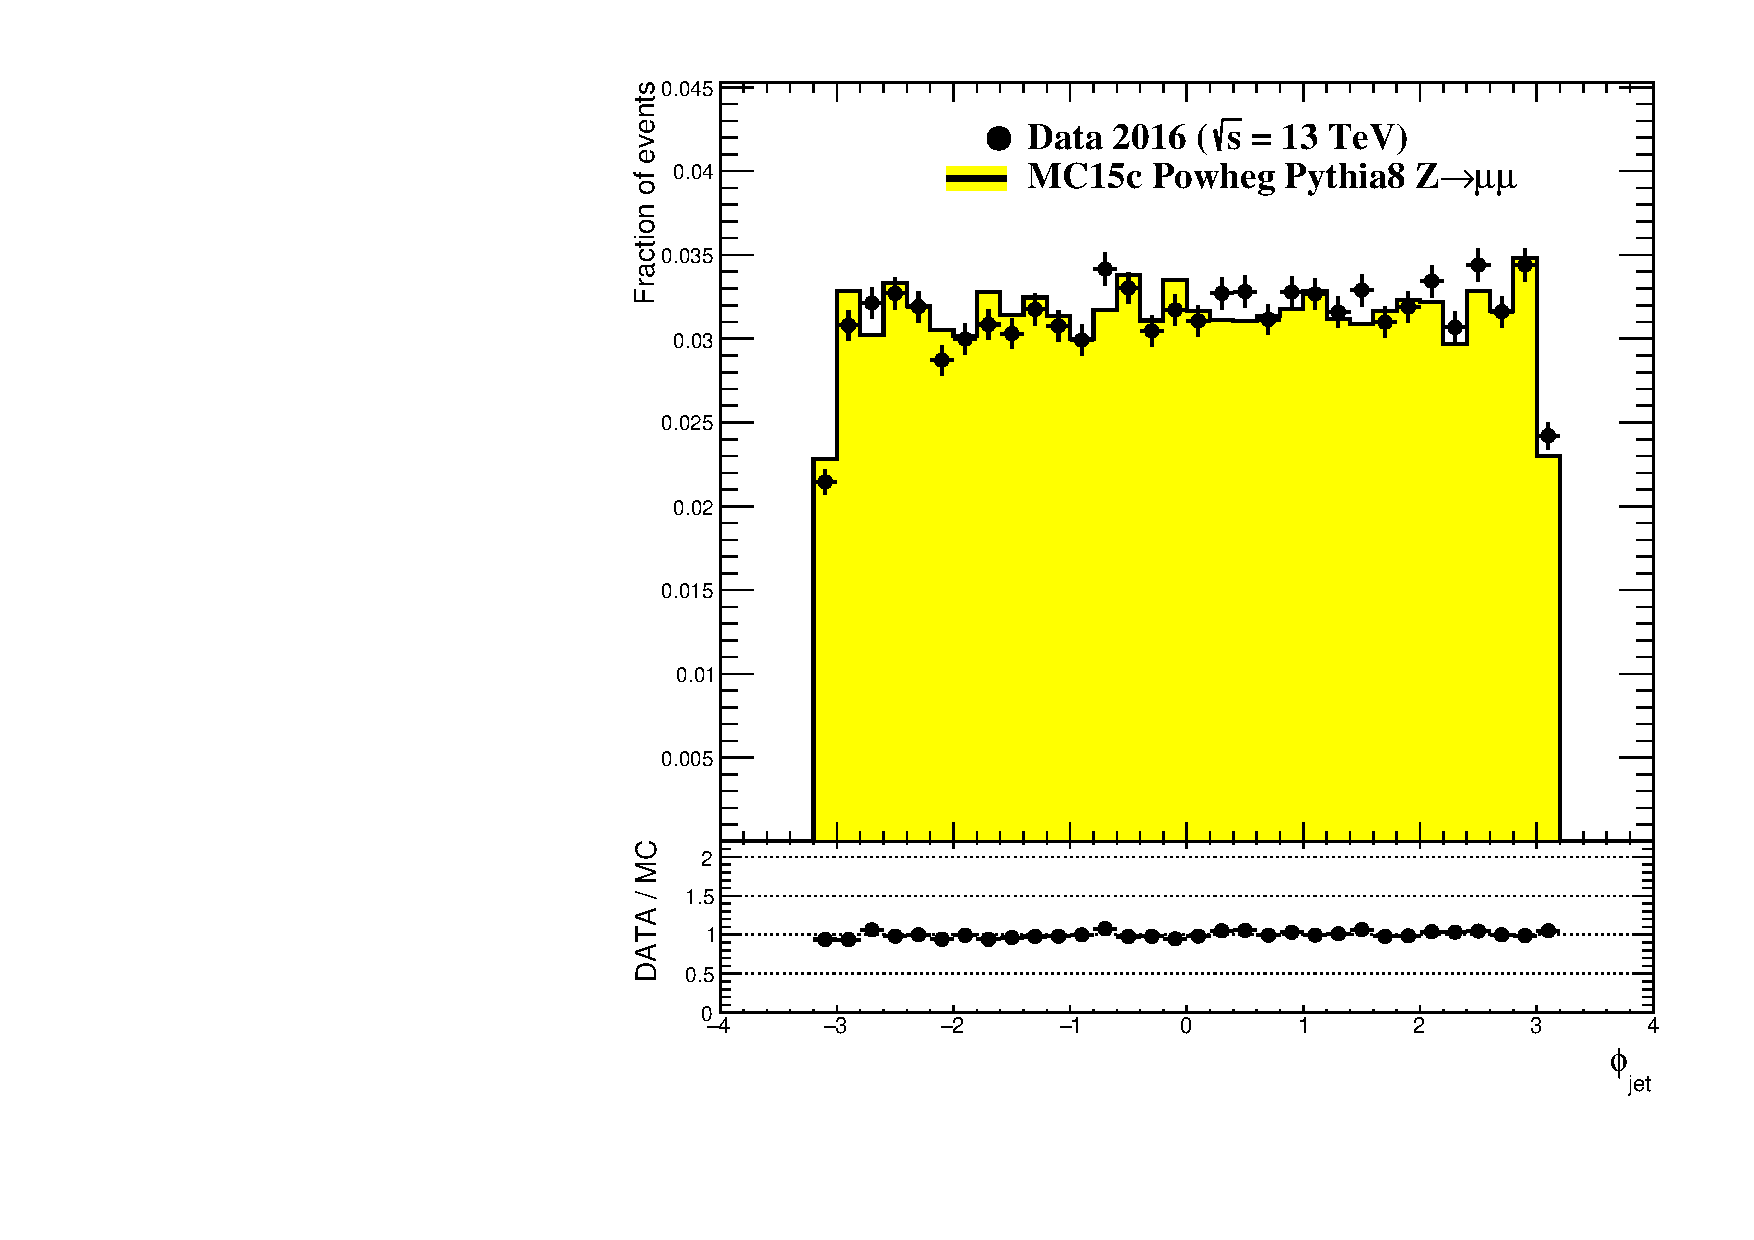
\includegraphics[width=0.53\figwidth]{jet_phiratio}
\caption[Influence of the Smearing on the energy]{The influence of the Smearing in energy is shown}
\label{fig:jetphi}
\end{subfigure}
\end{figure}

\section{Reconstruction of the Z-Boson}

The $Z-Boson$ is reconstructed as the vector-sum of the two muons in the selected event.
It is required to be in an range of \SI{90+-10}{\GeV} and to have a transversal momentum greater than \SI{30}{\GeV}.


\begin{figure}[h]
\centering
\begin{subfigure}[b]{0.5\figwidth}
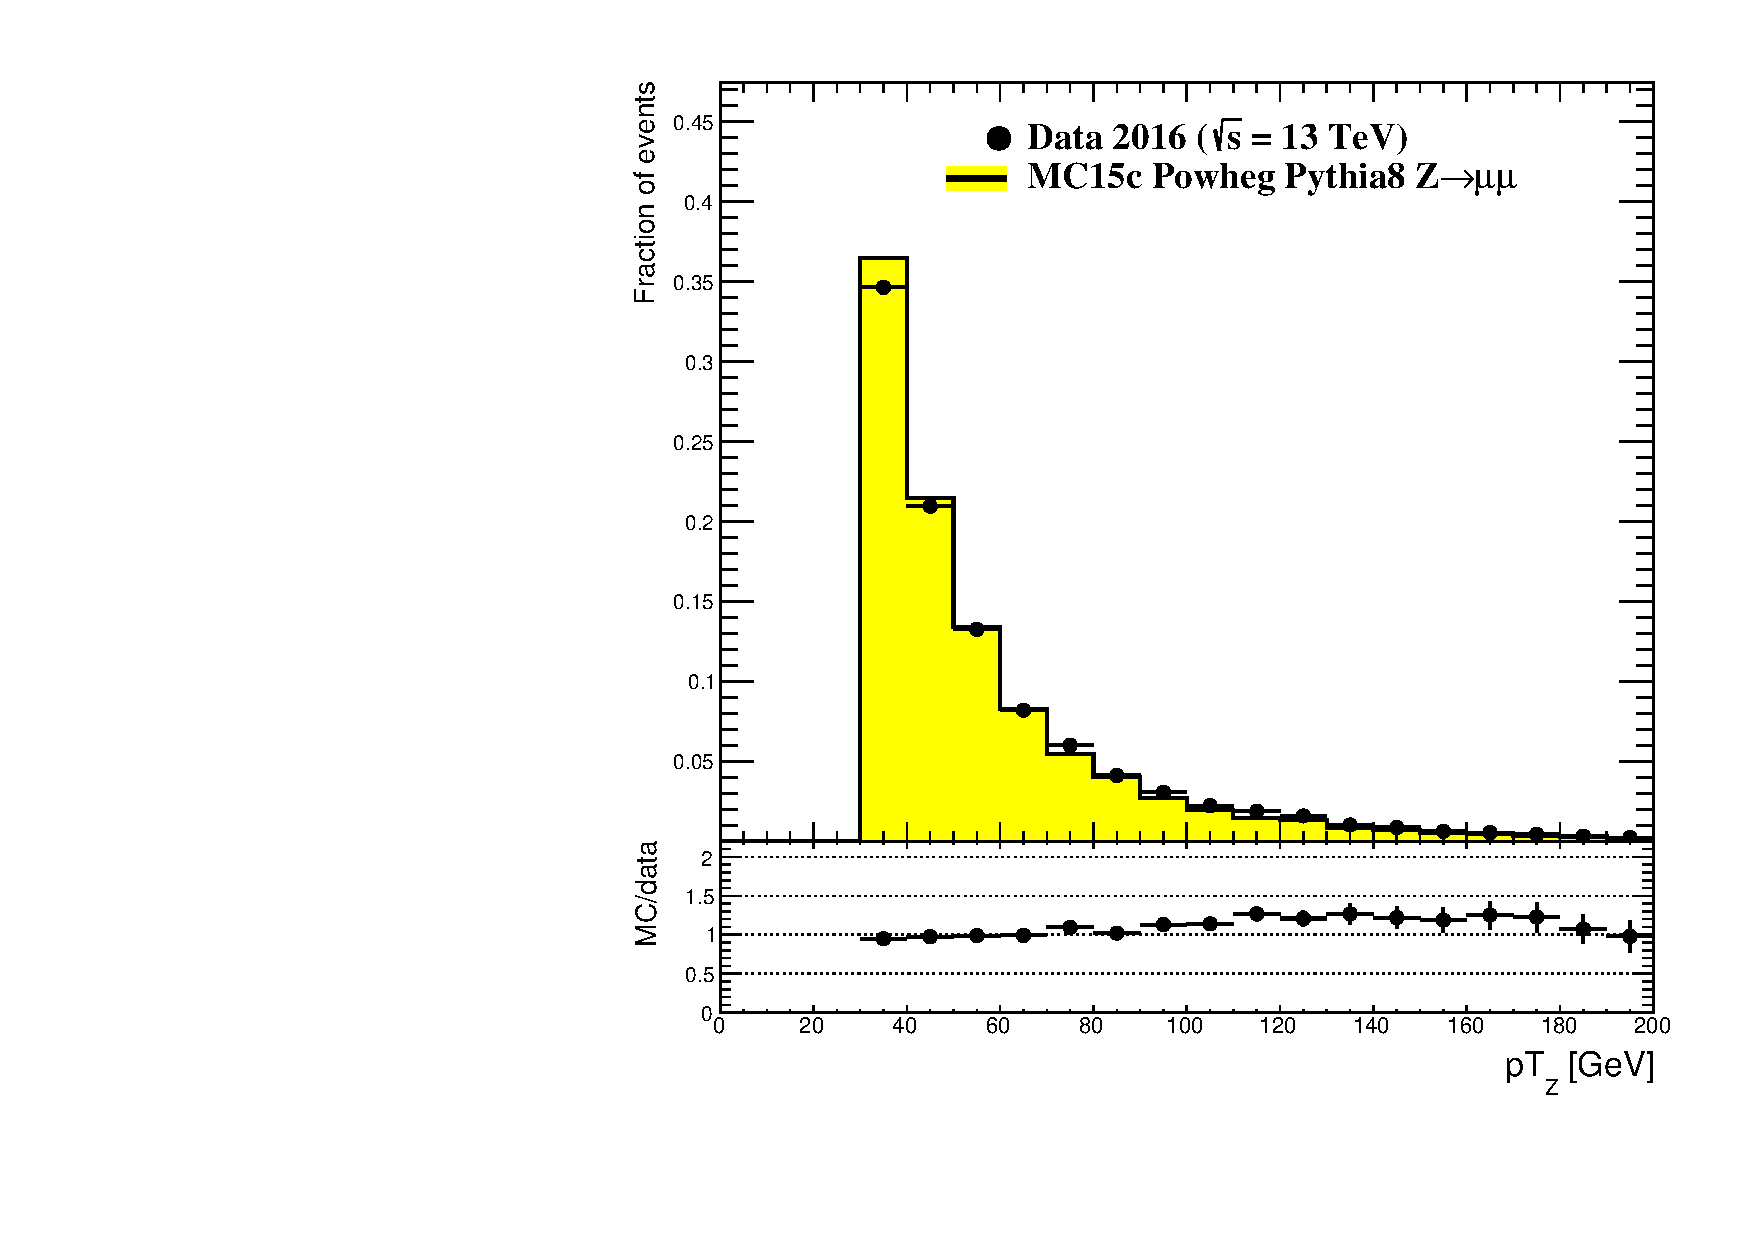
\includegraphics[width=0.53\figwidth]{Z_ptratio}
\caption[Influence of the JES on the transversal momentum]{The influence of the calibration in momentum is shown}
\label{fig:zpt}
\end{subfigure}
\quad
\begin{subfigure}[b]{0.5\figwidth}
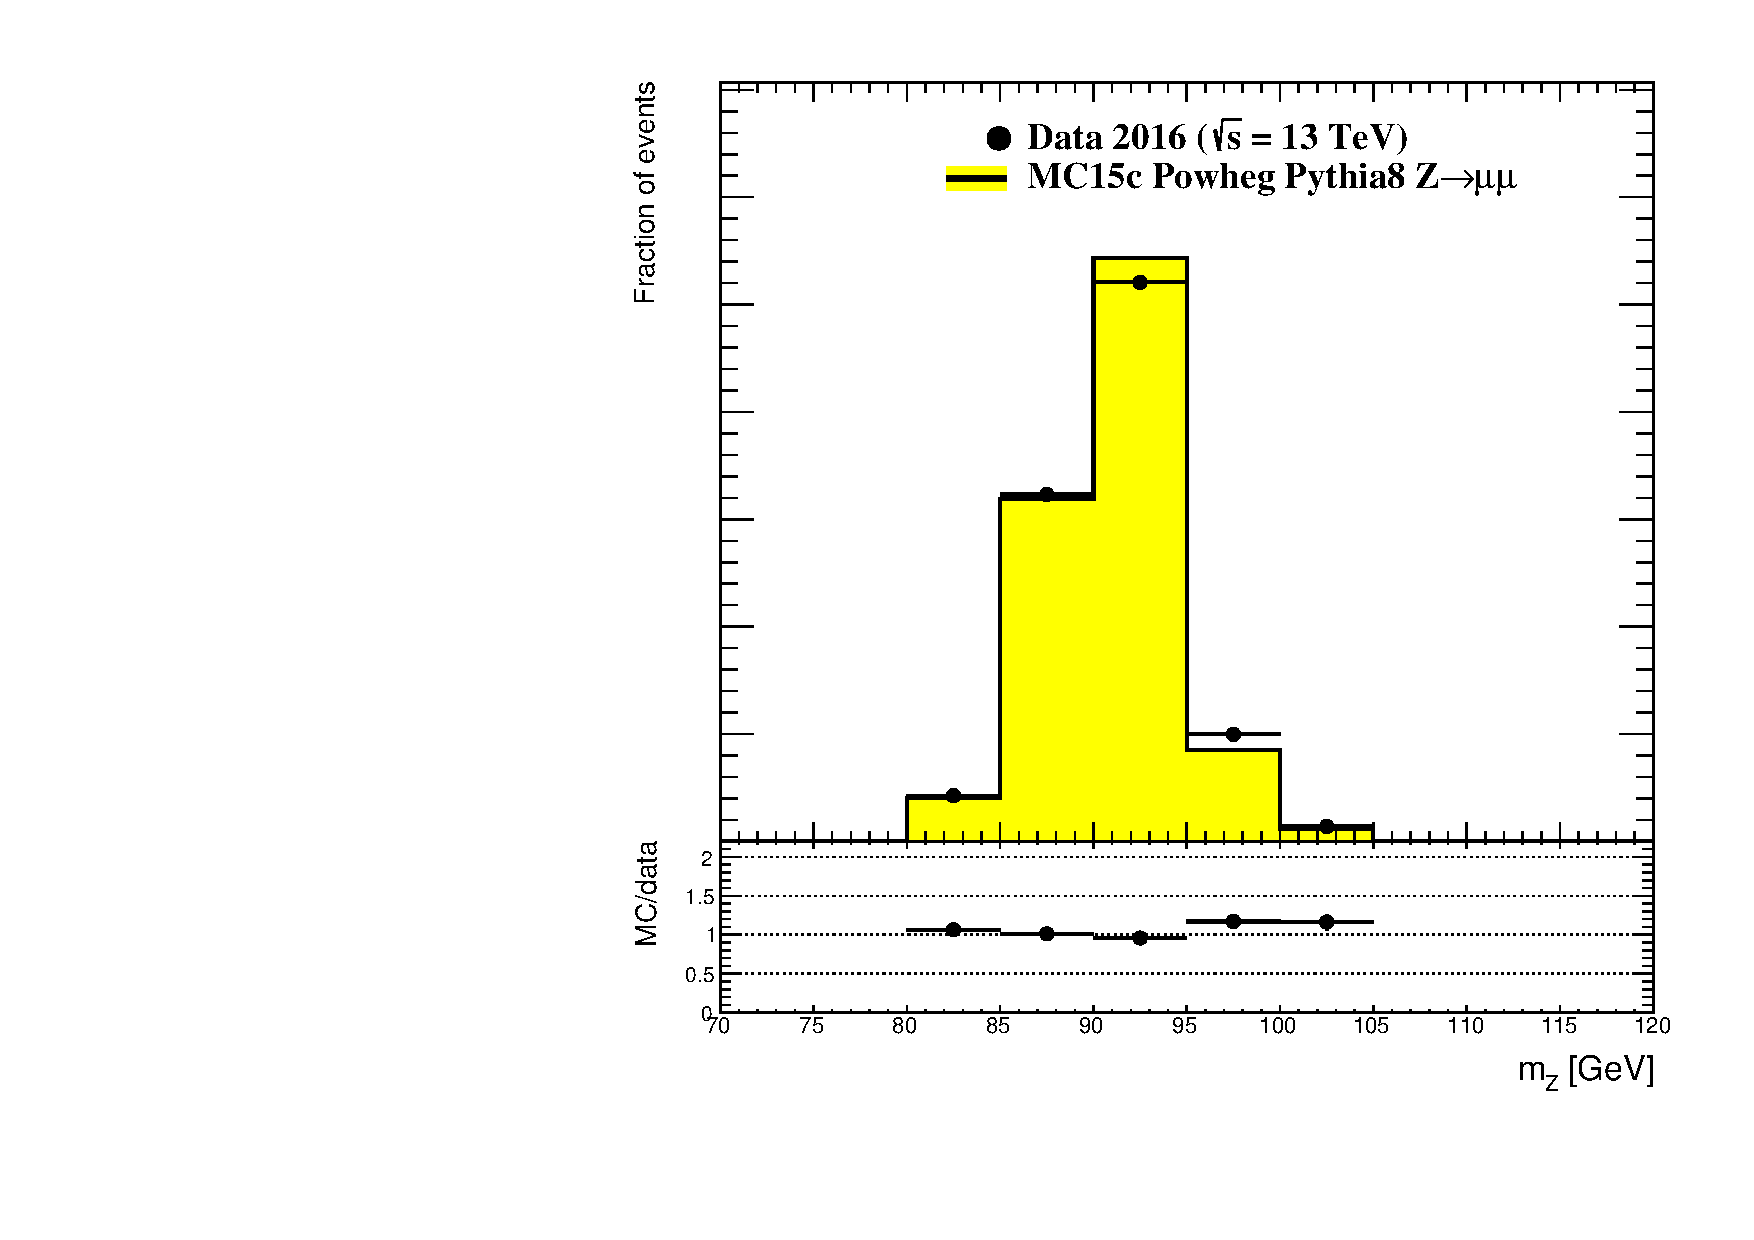
\includegraphics[width=0.53\figwidth]{Z_mratio}
\caption[Influence of the JES on the energy]{The influence of the calibration in energy is shown}
\label{fig:zm}
\end{subfigure}
\end{figure}


\begin{figure}[h]
\centering
\begin{subfigure}[b]{0.5\figwidth}
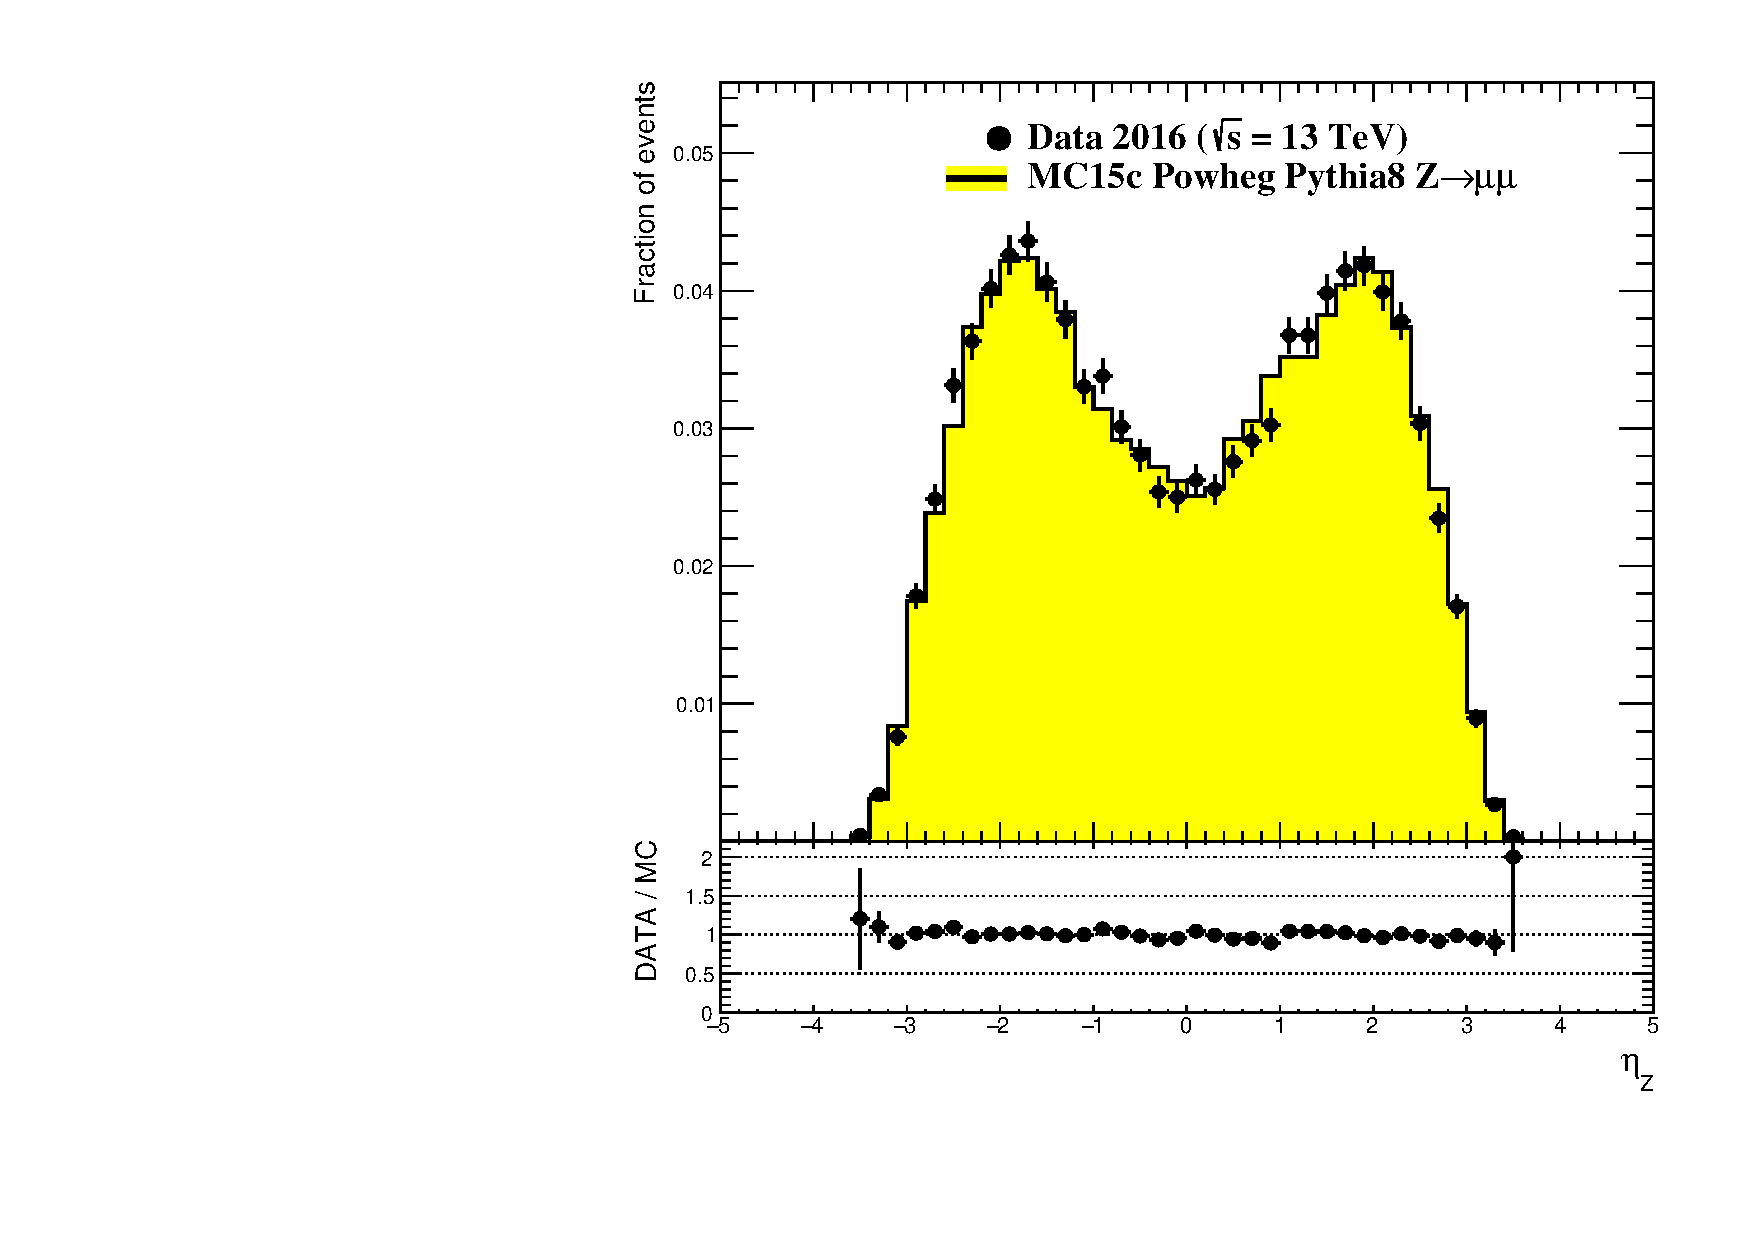
\includegraphics[width=0.53\figwidth]{Z_etaratio}
\caption[Influence of the Smearing on the transversal momentum]{The influence of the Smearing in momentum is shown}
\label{fig:zeta}
\end{subfigure}
\quad
\begin{subfigure}[b]{0.5\figwidth}
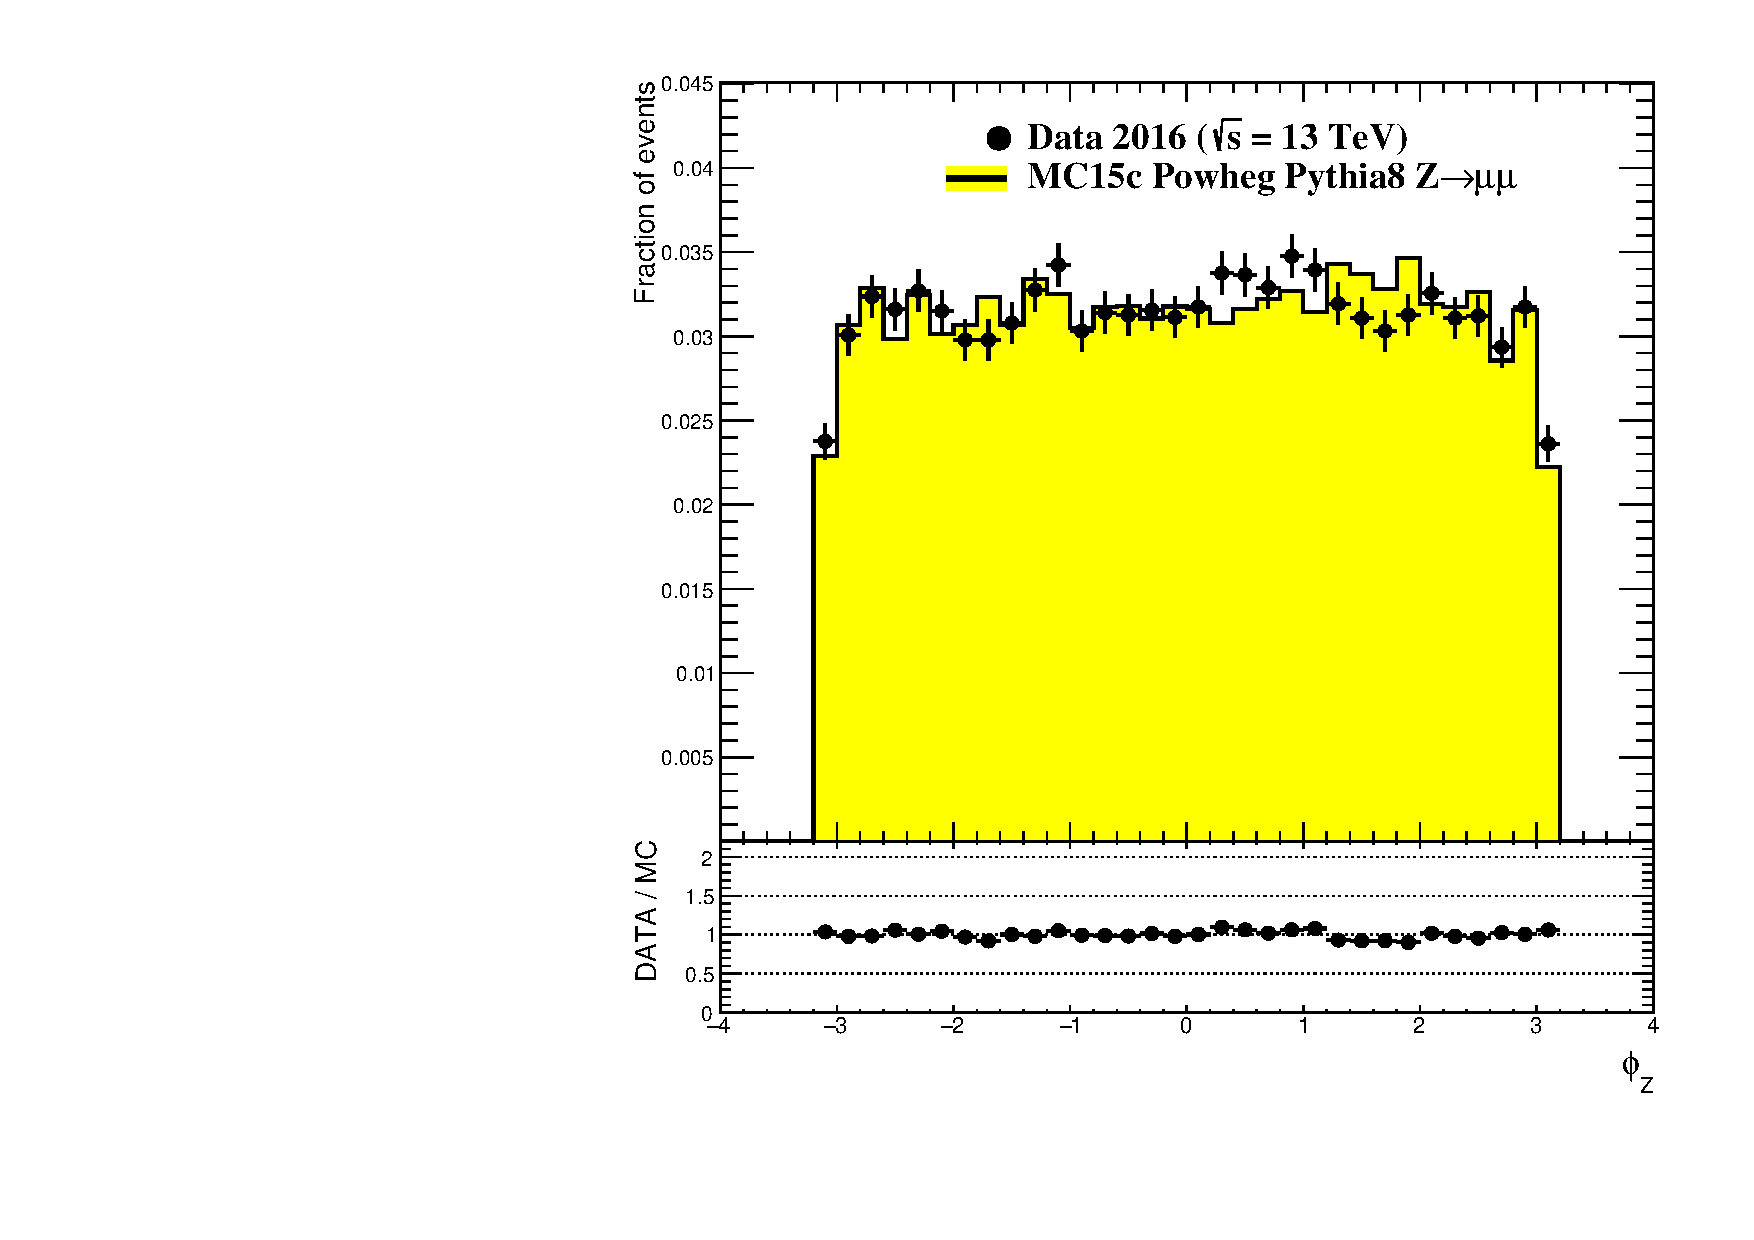
\includegraphics[width=0.53\figwidth]{Z_phiratio}
\caption[Influence of the Smearing on the energy]{The influence of the Smearing in energy is shown}
\label{fig:zphi}
\end{subfigure}
\end{figure}



\section{Performance of general variables}


The agreement between data and MC is good and can be expected to become promising well after testing with more statistics and also including all the scale factors and an individual cleaning for Partile Flow jets.

\begin{figure}[h]
\centering
\begin{subfigure}[b]{0.5\figwidth}
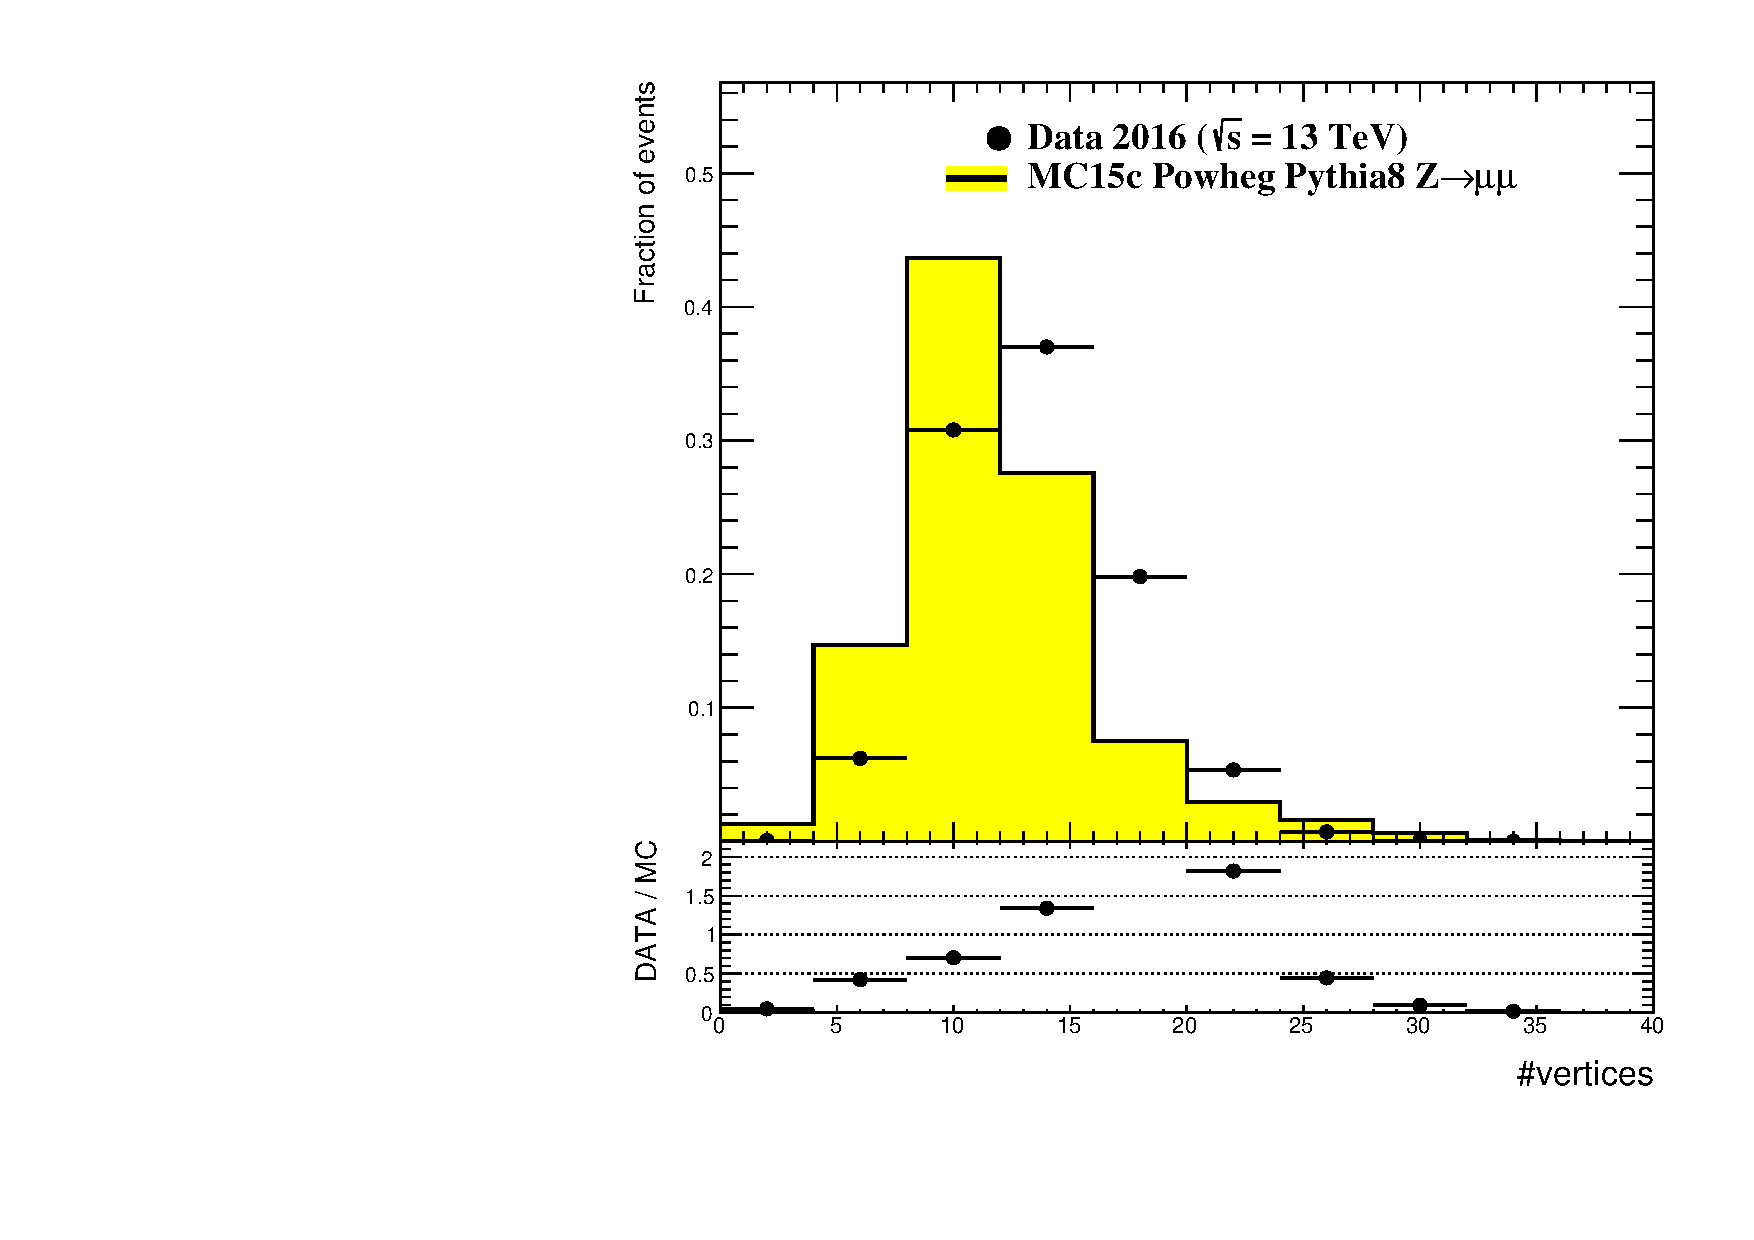
\includegraphics[width=0.53\figwidth]{verticesratio}
\caption[Influence of the JES on the transversal momentum]{The influence of the calibration in momentum is shown}
\label{fig:vertices}
\end{subfigure}
\quad
\begin{subfigure}[b]{0.5\figwidth}
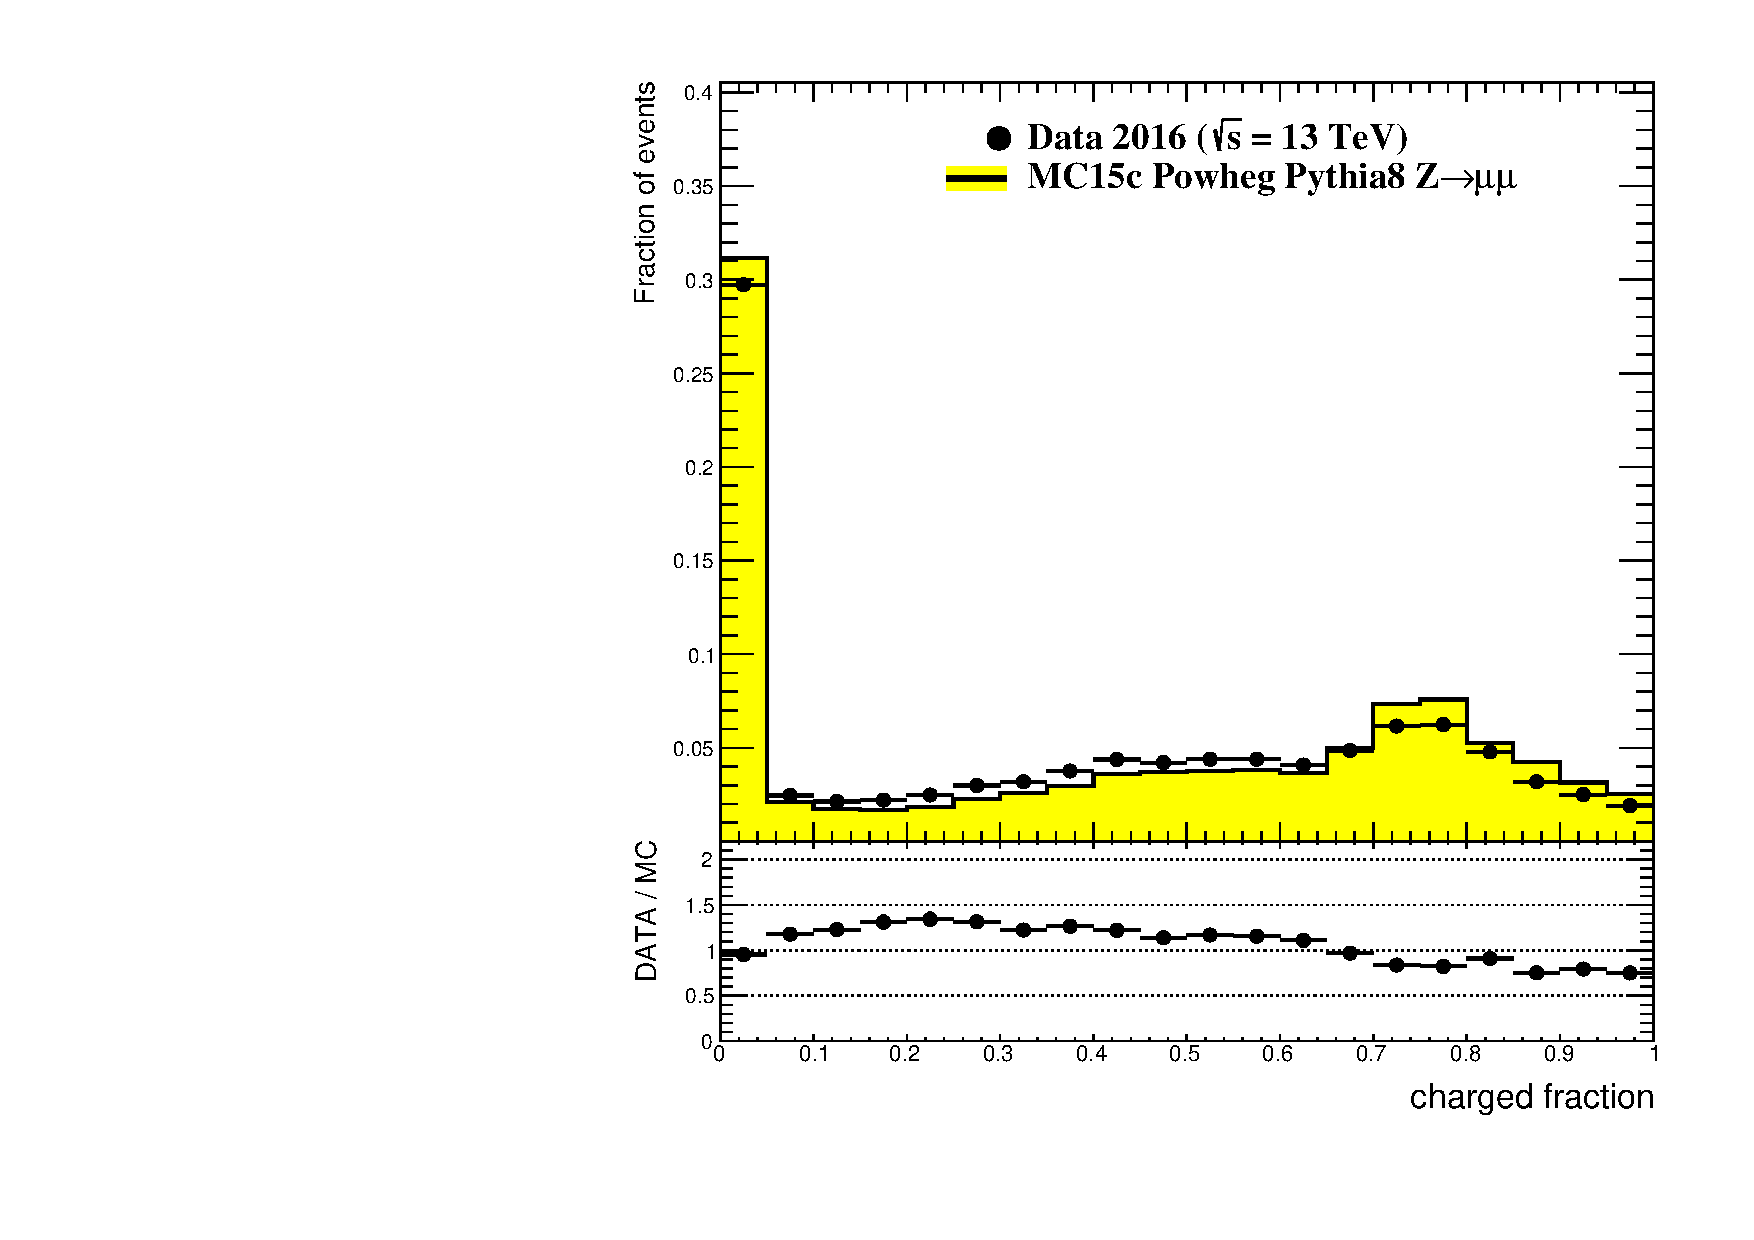
\includegraphics[width=0.53\figwidth]{chfracratio}
\caption[Influence of the JES on the energy]{The influence of the calibration in energy is shown}
\label{fig:chfrac}
\end{subfigure}
\end{figure}


\begin{figure}[h]
\centering
\begin{subfigure}[b]{0.5\figwidth}
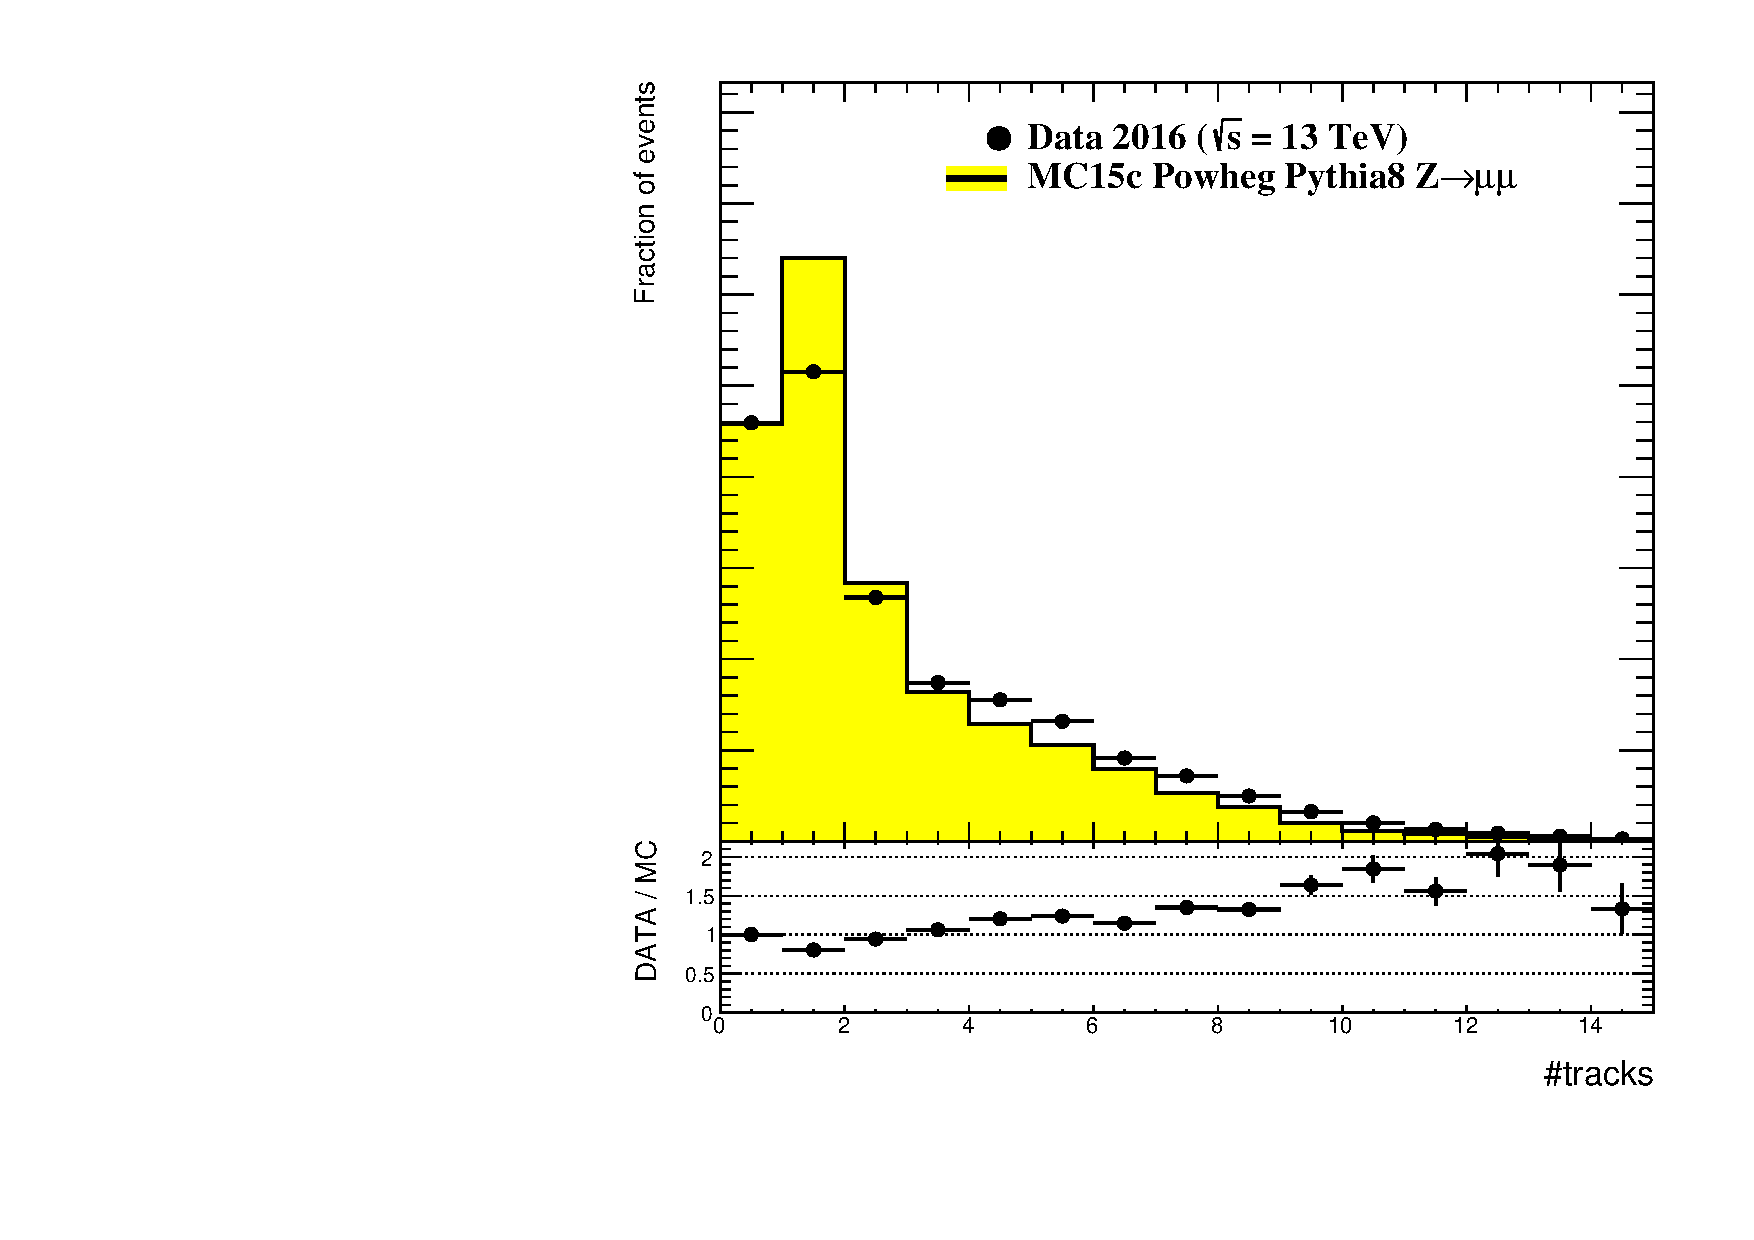
\includegraphics[width=0.53\figwidth]{trackcountratio}
\caption[Influence of the Smearing on the transversal momentum]{The influence of the Smearing in momentum is shown}
\label{fig:trackcount}
\end{subfigure}
\quad
\begin{subfigure}[b]{0.5\figwidth}
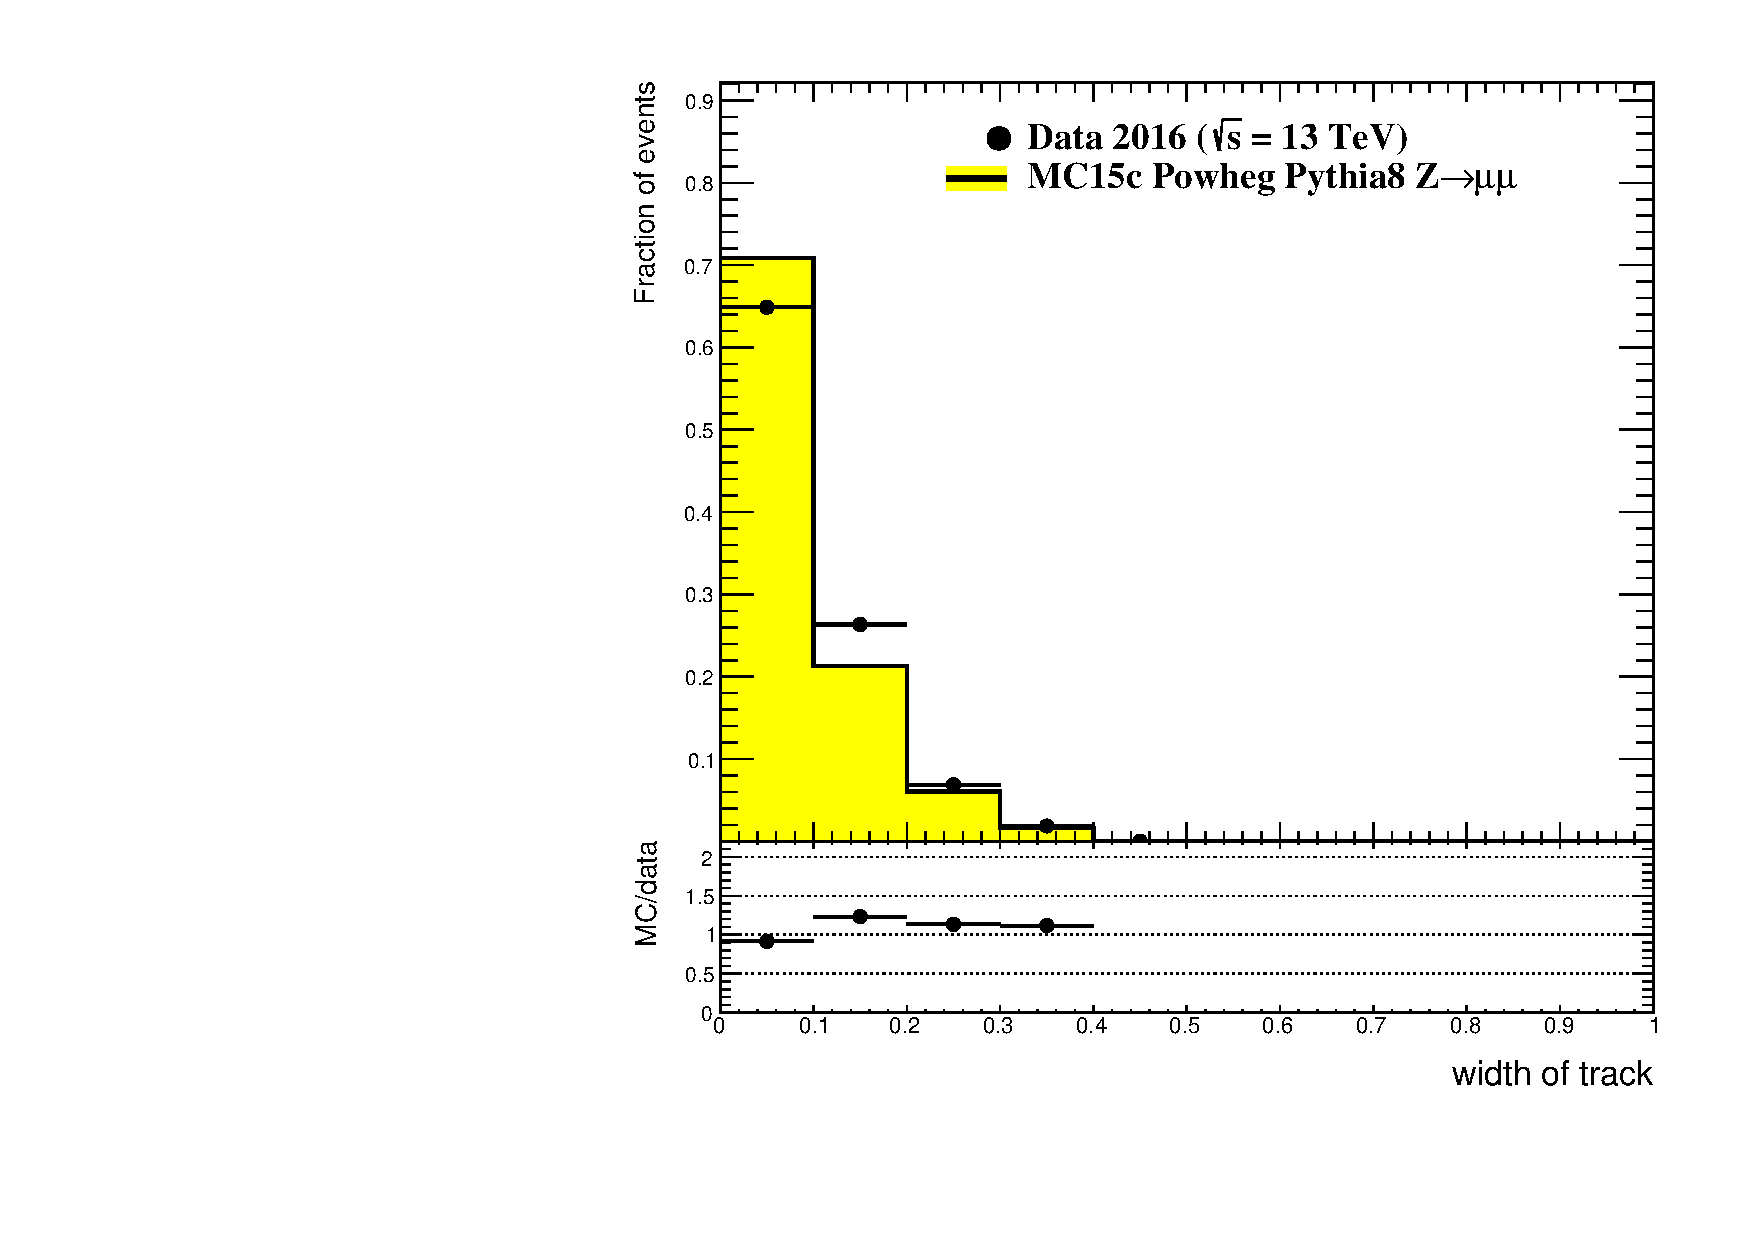
\includegraphics[width=0.53\figwidth]{trackwidthratio}
\caption[Influence of the Smearing on the energy]{The influence of the Smearing in energy is shown}
\label{fig:trackwidth}
\end{subfigure}
\end{figure}


\section{Data/Monte Carlo comparison}
\label{results}

I know nothing